\documentclass[12pt, a4paper]{report}
\setcounter{secnumdepth}{3} %subsubsections are numbered
\usepackage{caption}
\usepackage{graphicx}
\usepackage{hyperref}
\usepackage[dvipsnames]{xcolor}
\usepackage{tikz}
\usepackage{titlesec}
\counterwithin*{equation}{subsection}
\titleformat{\chapter}[hang]{\Huge\bfseries}{\thechapter -}{0pt}{\Huge\bfseries}
\renewcommand*\thesection{\arabic{section}}
\renewcommand{\thesubsubsection}{\thesubsection.\alph{subsubsection}}
\usepackage{amsmath, amsfonts, amssymb, amsthm}
\title{Logiske udsagn\\Opgaver}
\author{Kristoffer Klokker}
\date{2021}
\begin{document}
	\maketitle
	\tableofcontents
	\clearpage
	\setcounter{chapter}{35}	
	\chapter{Uge}
		\section{Afsnit 1.1}
			\subsection{1.1.1 -Which of these sentences are propositions? What are the truth values of those that are propositions?}
				\setcounter{subsubsection}{1}
				\subsubsection{Miami is the capital of Florida.}
					This is a proposition, due to the ability of being truth or false.\\
					The proposition is false the capital is Tallahassee
				\setcounter{subsubsection}{2}
				\subsubsection{5 + 7 = 10.}
					The is a proposition, but false.
				\setcounter{subsubsection}{5}
				\subsubsection{Answer this question.}
					This is not a proposition due to its inability to be true or false.
			\setcounter{subsection}{12}
			\subsection{1.1.13 - Let p and q be the propositions - p: It is below freezing. \& q: It is snowing. Write these propositions using p and q and logical connectives (including negations).}
				\setcounter{subsubsection}{1}
				\subsubsection{It is below freezing but not snowing}
					$p \land \neg q$
				\setcounter{subsubsection}{2}
				\subsubsection{It is either snowing or below freezing (or both).}
					$p \lor q$
				\setcounter{subsubsection}{5}
				\subsubsection{Either it is below freezing or it is snowing, but it is not snowing if it is below freezing.}
					$p \oplus q$
\setcounter{subsection}{30}
			\subsection{1.1.31 - How many rows appear in a truth table for each of these compound propositions?}
\setcounter{subsubsection}{2}
				\subsubsection{$q\lor p \lor \neg s \lor \neg r \lor \neg t \lor u$}
					10 - one for each variable and the negated variable and the final column.\\
					Since all are or is it easy to read due to only one is needed to be true.
				\subsubsection{$(p\land r \land t) \iff ( q\land t)$}
					7 - one of each variable, parenthesis and the final column.

\setcounter{subsection}{32}
			\subsection{1.1.33 - Construct a truth table for each of these compound propositions}

\setcounter{subsubsection}{1}
				\subsubsection{$p\lor \neg q$}
					\begin{table}[h!]
						\begin{tabular}{|l|l|l|l|}
						\hline
						$p$ & $q$ & $\neg q$ & $p \lor \neg q$ \\ \hline
						T   & T   & F        & T               \\ \hline
						T   & F   & T        & T               \\ \hline
						F   & T   & F        & F               \\ \hline
						F   & F   & T        & T               \\ \hline
					\end{tabular}
					\end{table}

\setcounter{subsubsection}{3}
				\subsubsection{$(p\lor q)\implies (p\land q)$}
					\begin{table}[h!]
						\begin{tabular}{|l|l|l|l|l|}
						\hline
						$p$ & $q$ & $p\lor q$ & $p \land q$ & $(p\lor q) \implies (p\land q)$ \\ \hline
						T   & T   & T         & T           & T                               \\ \hline
						T   & F   & T         & F           & F                               \\ \hline
						F   & T   & T         & F           & F                               \\ \hline
						F   & F   & F         & T           & T                               \\ \hline
						\end{tabular}
					\end{table}
		\section{Afsnit 1.3}
			\setcounter{subsection}{6}
			\subsection{1.3.7 Use De Morgan’s laws to find the negation of each of the following statements.}
			
\setcounter{subsubsection}{2}

				\subsubsection{c - Mei walks or takes the bus to class.}
					p: Mei walks to class\\
					q: Mei talkes the buss to class\\
					$p \lor q$\\
					$\neg( p \lor q)$\\
					$\neg p \land \neg q$
				\subsubsection{d - Ibrahim is smart and hard working.}
					p:  Ibrahim is smart\\
					q:  Ibrahim is hard working\\
					$p \land q$\\
					$\neg( p \land q)$\\
					$\neg p \lor \neg q$

			\setcounter{subsection}{18}
			\subsection{1.3.19 Determine whether $(\neg q \land (p \implies q)) \implies \neg p$ is a tautology. Each of Exercises 20–32 asks you to show that two compound propositions are logically equivalent. To do this, either show that both sides are true, or that both sides are false, for exactly the same combinations of truth values of the propositional variables in these expressions (whichever is easier).}
				To make the expression false the right side of the implication has to be false which is done by making $p$ true.\\
				The left side has to be true, but that is not possible because for the implication to be true $q$ has to be true.\\
				But by making $q$ true the and will result in false due to the negation.\\
				Tnerefore it is a tautology.
		\section{Hvilke af følgende udsagn er sande?}
			\subsection{Hvis $p$ er falsk, er $\neg p \lor q$ sand.}
				Sandt
			\subsection{$p\lor q$ er sand, hvis og kun hvis $p$ er sand.}
				Falsk
			\subsection{Hvis $p\land q$ er sand, er $p\lor q$ også sand.}
				Sandt
			\subsection{Hvis $p\implies q$ er sand, og $q$ er falsk, er $p$ også falsk}
				Sandt
			\subsection{Hvis $p$ er falsk, kan $q$ tildeles en sandhedsværdi, sådan at $p\lor \neg q$ er sand.}
				Sandt - $q$ = falsk
		\setcounter{section}{0}
		\section{Angiv for hvert af de føægende par af udsagn om $(a)\implies (b), (b)\implies (a), (a)\iff (b)$ eller inge n af delene.}
			\subsection{$(a) p\lor q | (b) p \land q$}
				$(b)\implies (a)$
			\subsection{$(a)\neg p \lor q | (b) p\implies q$}
				$(a)\iff(b)$

		\section{Afsnit 1.4}			
			\setcounter{subsection}{4}
			\subsection{Opgave 1.4.5 Let P(x) be the statement “x spends more than five hours every weekday in class,” where the domain for x consists of all students. Express each of these quantifications in English}
				\subsubsection{$\exists x P(x)$}
					There exists students who spends more than fice hours every weekday in class
				\subsubsection{$\forall x P(x)$}
					All students use spends more than five hours every weekday in class
				\subsubsection{$\exists x\neg P(x)$}
					There exists student who does not use more than five hours every weekday in class
				\subsubsection{$\forall x \neg P(x)$}
					No student use more than five hours in class every weekday in class
			\setcounter{subsection}{10}
			\subsection{Opgave 1.4.11 Let P(x) be the statement $x = x2$. If the domain consists of the integers, what are these truth values?}
				\subsubsection{$P(0)$}
					True
				\subsubsection{$P(1)$}
					False
				\subsubsection{$P(2)$}
					False
				\subsubsection{$P(-1)$}
					False
				\subsubsection{$\exists x P(x)$}
					True
				\subsubsection{$\forall x P(x)$}
					False
			\subsection{As mentioned in the text, the notation $\exists!xP(x)$ denotes “There exists a unique x such that P(x) is true.” If the domain consists of all integers, what are the truth values of these statements?}
				\subsubsection{$\exists!x(x>1$}
					False
				\subsubsection{$\exists!x(x^2=1)$}
					True
	\chapter{Uge}
		\section{Angiv for hvert af de følgende par af udsagn om $(a)\implies (b), (b)\implies (a), (a)\iff (b)$ eller ingen af delene}
			\subsection{$(a) \neg(p\land q) | (b) p\lor q$}
				Det er ingen af delene.
			\subsection{$(a) (p\lor q)\land (p \lor r) | (b) p\lor (q\land r)$}
				$(a)\iff(b)$ 
			\subsection{$(a) \neg p\implies q | (b) \neg q \implies p$}
				$(a)\iff (b)$
		\section{Afsnit 1.4}
			\setcounter{subsection}{15}
			\subsection{Opgave 1.4.16: Determine the truth value of each of these statements if the domain of each variable consists of all real numbers.}
				\subsubsection{$\exists x (x^2=2)$}
					True - $x=\sqrt{2}$
				\subsubsection{$\exists x (x^2=-1)$}
					False
				\subsubsection{$\forall x (x^2+2\leq 1)$}
					True
				\subsubsection{$\forall x (x^2 \neq x)$}
					False - $x=0$
			\setcounter{subsection}{53}
			\subsection{Opgave 1.4.54: As mentioned in the text, the notation $\exists !xP(x)$ denotes “There exists a unique x such that P(x) is true.” If the domain consists of all integers, what are the truth values of these statements?}
				\subsubsection{$\exists ! x (x+3=2x)$}
					Sandt - $x=3$
				\subsubsection{$\exists ! x (x=x+1)$}
					Falsk
			\setcounter{subsection}{61}
			\subsection{Opgave 1.4.62: Let $P(x), Q(x)$, and $R(x)$ be the statements “x is a clear explanation,” “x is satisfactory,” and “x is an excuse,” respectively. Suppose that the domain for x consists of all English text. Express each of these statements using quantifiers, logical connectives, and $P(x), Q(x)$, and$ R(x)$.}
				\subsubsection{All clear explanations are satisfactory.}
					$\forall x (P(x) \implies Q(x))$
				\subsubsection{Some excuses are unsatisfactory.}
					$\exists x( R(x) \land \neg Q(x))$
				\subsubsection{Some excuses are not clear explanations.}
					$\exists x (R(x) \land \neg P(x))$
				\subsubsection{Does (c) follow from (a) and (b)? - $(a)\land (b)\implies (c)$}
					\begin{align}
						\forall x: P(x)\implies q(x) \land \exists x : r(x) \land \neg Q(x)\\
						\exists x : (P(x)\implies Q(x))\land(R(x) \land \neg Q(x))\\
						\exists x : (\neg P(x)\lor Q(x))\land (R(x)\land \neg Q(x))\\
						\exists x : (\neg P(x)\lor Q(x)\land R(x)\land \neg Q(x)\\
						\exists x : \neg P(x)\land R(x)
					\end{align}
					1-2 bliver udtrykket mindre stærkt. 4-5 Q skal være falsk og dermed går det ud.
		\setcounter{section}{0}
		\section{Afsnit 1.5}
			\setcounter{subsection}{8}
			\subsection{Opgave 1.5.9: Let $L(x, y)$ be the statement “x loves y,” where the domain for both x and y consists of all people in the world. Use quantifiers to express each of these statements.}
				\subsubsection{Everybody loves Jerry}
					$\forall x (L(x,"Jerry"))$
				\subsubsection{Everybody loves somebody}
					$\forall x: \exists y: L(x,y)$
			\setcounter{subsection}{18}
			\subsection{Opgave 1.5.19: Express each of these statements using mathematical and logical operators, predicates, and quantifiers, where the domain consists of all integers.}
				\subsubsection{The sum of two negative intergers is negative}
					$\forall x,y \in \mathbb{Z}^-: x+y <0$	
				\subsubsection{The difference of two positive intergers is not necessarily positive}
					$\exists x,y \in \mathbb{Z}^+: x-y < 0$
			\setcounter{subsection}{26}
			\subsection{Opgave 1.5.27: Determine the truth value of each of these statements if the domain for all variables consists of all integers.}
				\subsubsection{$\forall n \exists m(n^2 <m)$}
					Sandt	
				\subsubsection{$\exists n \forall m(n<m^2)$}
					Sandt - $n\leq 0$
				\subsubsection{$\forall n \exists m(n+m=0)$}
					Sandt - $m=-n$
			\setcounter{subsection}{29}
			\subsection{ Opgave 1.5.30: Rewrite each of these statements so that negations appear only within predicates (that is, so that no negation is outside a quantifier or an expression involving logical connectives).}
				\subsubsection{$\neg\forall x\exists y  P(x,y)$}	
					$\exists x \forall y \neg p(x,y)$
			\setcounter{subsection}{38}
			\subsection{Opgave 1.5.39: Find a counterexample, if possible, to these universally quantified statements, where the domain for all variables consists of all integers.}
				$\forall x \forall y (x^2=y^2\rightarrow x= y)$
				Let x be minus y 
			\setcounter{subsection}{0}
			\subsection{Opgave 1.7.1: Use a direct proof to show that the sum of two odd inte			gers is even.}
				\begin{align*}
					o: odd(2x+1)\\
					e: even(2x)\\
					o+o=4x+2
				\end{align*}
			\setcounter{subsection}{17}
			\subsection{Opgave 1.7.18: Prove that if m and n are integers and mn is even, then m is even or n is even.}
				\begin{align*}
					o: odd(2x+1)\\
					e: even(2x)\\
					o\cdot o =2x^2+2x+2x+1=2x^2+4x+1\\
					e\cdot o = 4x^2+2x\\
					e\cdot e = 4x^2
				\end{align*}
					It is seen that two odds multiplied is still odd and in any other case its even.\\
		\section{Lad $n\in\mathbb{N}$ og lad $P(n)$ være udsagnet $$\sum^n_{i=0}3^i=\frac{3^{n+1}-1}{2}$$Opgaven går ud på at bevise, at P (n) er sand for alle $n \in N$, ved hjælp af induktion.}
			\subsection{Hvad er udsagnet $P(0)$?}
				$P(0)=\sum^0_{i=0}3^i=\frac{3^{0+1}-1}{2}=1$
			\subsection{Opskriv induktionsantagelsen}
				$\sum^{n+1}_{i=0}3^i=\frac{3^{(n+1)+1}-1}{2}$\\
				\begin{align*}
					P(k): \sum_{i=0}^k3^i&=\frac{3^{k+1}-1}{2}\\
					P(k+1): \sum_{i=0}^{k+1}3^i&=\frac{P3^{k+2}-1}{2}\\
				\sum_{i=0}^{k+1}3^i&=\sum_{i=0}^k3^i+3^{k+1}\\
						   &=\frac{3^{k+1}-1}{2}+3^{k+1}\\
						   &=\frac{3^{k+1}-1}{2}+\frac{2\cdot 3^{k+1}}{2}\\
						   &=\frac{3\cdot 3^{k+1}-1}{2}\\
						   &=\frac{3^{k+2}-1}{2}
				\end{align*}
		\setcounter{section}{0}
		\section{Afsnit 1.5}
			\setcounter{subsection}{10}
			\subsection{Opgave 5.1.11: Find a formula for $\frac{1}{2}+\frac{1}{4}+\frac{1}{8}...\frac{1}{2^n}$ by examining the values of this expression for small values of n. And Prove the formula you conjectured.}
				$p(n)=\frac{1}{n(n+1)}$\\
				$p(1)=\frac{1}{1(1+1)}=\frac{1}{2}$\\
				$p(n+1)=\frac{1}{n(n+1)}+\frac{1}{2^{n+1}}$\\
				$p(n+1)=\frac{1+n(n+1)}{n(n+1)+2^{n+1}}$\\
				$p(n+1)=\frac{1+n^2+n}{n^2+n+2^{n+1}}$
			\setcounter{subsection}{8}
			\subsection{Opgave 1.5.9: Let L(x, y) be the statement “x loves y,” where the domain for both x and y consists of all people in the world. Use quantifiers to express each of these statements.}
				\subsubsection{There is somebody whom everybody loves.}
					$\exists y \forall x l(x,y)$
				\subsubsection{Nobody loves everybody.}
					$\exists x \forall y\neg p(x,y)$
			\setcounter{subsection}{18}

			\subsection{1.5.19: Express each of these statements using mathematical and logical operators, predicates, and quantifiers, where the domain consists of all integers.}
				\subsubsection{The sum of the squares of two integers is greater than or equal to the square of their sum.}
					$\forall x \forall y \in \mathbb{Z}: \sqrt{x}+\sqrt{y}\geq \sqrt{x+y}$
				\subsubsection{The absolute value of the product of two integers is the product of their absolute values}
					$\forall x \forall y \in \mathbb{Z}: |x|\cdot |y|=|x\cdot y|$
			\setcounter{subsection}{26}
			\subsection{1.5.27: Determine the truth value of each of these statements if the domain for all variables consists of all integers}
				\subsubsection{$\exists n \forall m (nm=m)$}
					True - n = 1
				\subsubsection{$\exists n \exists m (n^2+m^2=5)$}
					True - n =1 and m = 2
				\subsubsection{$\exists n \exists m(n^2+m^2=6)$}
					False
				\subsubsection{$\forall n \forall m \exists p (p=(m+n)/2)$}
					False - p will not be an integer
					\subsection{1.5.30: Rewrite each of these statements so that negations appear only within predicates (that is, so that no negation is outside a quantifier or an expression involving logical connectives).}
				\subsubsection{$\neg\exists y \exists x P(x,y)$}
					$\forall y \forall x \neg P(x,y)$
				\subsubsection{$\neg \forall x \exists y P(x,y)$}
					$\exists x \forall y \neg P(x,y)$
			\setcounter{subsection}{38}
			\subsection{1.5.39: Find a counterexample, if possible, to these universally quantified statements, where the domain for all variables consists of all integers.}
				\subsubsection{$\forall x \exists y (y^2=x)$}
					If x is a prime number.
				\subsubsection{$\forall x \forall y (xy \geq x)$}
					If y is 0
		\section{Afsnit 1.7}
			\setcounter{subsection}{5}
			\subsection{1.7.6: Use a direct proof to show that the product of two odd numbers is odd.}
				\begin{align*}
					o: odd(2x+1)\\
					o\cdot o=(2x+1)\cdot(2x+1)=4x^2+4x+1
				\end{align*}
			\setcounter{subsection}{28}
				\subsection{1.7.29: Prove that if n is a positive integer, then n is odd if and only if 5n + 6 is odd.}
					\begin{align*}
						e: even(2x)\\
						o: odd(2x+1)\\
						5e+6=10x+6\\
						5o+6=10x+11
					\end{align*}
		\setcounter{section}{0}
		\section{Afsnit 1.7}
			\setcounter{subsection}{4}
			\subsection{1.7.5: Prove that if $m + n$ and $n + p$ are even integers, where $m, n, and p$ are integers, then $m + p$ is even. What kind of proof did you use?}
				Due to only even intergeres beign used in a plus operation, a odd integer is not possible to create, due to a plus operation needing a odd integer to result in an odd integer.\\
				Exhaustive proof, to some kind.
			\setcounter{subsection}{35}
			\subsection{1.7.36: Is this reasoning for finding the solutions of the equation $\sqrt{2x^2 - 1} = x$ correct? (1) $\sqrt{2x^2 - 1} = x$ is given; (2) $2x^2 - 1 = x^2$ , obtained by squaring both sides of (1);(3) $x^2 - 1 = 0$, obtained by subtracting $x^2$ from both sides of (2); (4) $(x - 1)(x + 1) = 0$, obtained by factoring the left-hand side of $x^2 - 1$; (5) $x = 1$ or $x = -1$, which follows because $ab = 0$ implies that $a = 0$ or $b = 0$.}
				Yes it a direct proof of a solution.
			\setcounter{subsection}{42}
			\subsection{1.7.43: Prove that if n is an integer, these four statements are equivalent: (i) n is even, (ii) $n + 1$ is odd, (iii) $3n + 1$ is odd, (iv) $3n$ is even}
				\begin{align*}
					e: even(2x)\\
					o: odd(2x+1)\\
					n = e\\
					n+1=e+1=2x+1=o\\
					3n+1=3(2x)+1=6x+1=o\\
					3n=3(2x)=6x=e
				\end{align*}
		\section{Afsnit 1.8}
			\setcounter{subsection}{10}
			\subsection{1.8.11: Suppose that in a four-round obligato game, the teacher first gives the student the proposition $\neg(p \implies (q \land r))$, then the proposition $p \lor\neg q$, then the proposition $\neg r$, and finally, the proposition $(p \land r) \lor (q \implies p)$. For which of the 16 possible sequences of four answers will the student pass the test?}
			$\neg(p\implies (q\land r))$\\
			q = sand\\
			$p\lor\neg q$\\
			p = sand\\
			$\neg r$\\
			r = falsk\\
			$(p\land r)\lor(q\implies p)$\\
		\section{Afsnit 5.1}
			\setcounter{subsection}{17}
			\subsection{5.1.18: Let P(n) be the statement that $n! < n^n$ , where n is an integer greater than 1}
				\subsubsection{What is hte statement P(2)}
				$2!<2^2\iff 2<4$
				\subsubsection{Show that $P(2)$ is true, completing the basis step of proof by mathimatical induction that $P(n)$ is true for all integers $n$ gratger than 1.}
				-||-
				\subsubsection{What is the inductive hypothesis of a proof by mathimatical induction that $P(n)$ is true for all integers $n$ grather than 1?}
	\chapter{Uge}
		\section{Afsnit 1.8}
			\setcounter{subsection}{31}
			\subsection{ Opgave 1.8.32: Prove that there are no solutions in integers x and y to the equation $2x^2 + 5y^2 = 14$.}
				Udtrykket kan reduceres til $x^2+2.5y^2=7$\\
				Herfra kan det ses at begge variabler har eksponenten 2 og da de to variabler bliver adderet kan det muligt at lave et exhaust bevis.\\
				$x^2$ vil her kunne have følgende værdier når $x$ er en integer under 7: $0,1,2,4$\\
				Ligesådan vil $2.5y^2$ have følgende værdier under 7: $0,2.5$\\
				Det kan her ses at der ikke er nogle mulige kombinationer som ved en addition vil give 7 og dermed er der ingen løsning.
		\section{Afsnit 5.1}
			\setcounter{subsection}{9}
			\subsection{Opgave 5.1.10}
				\subsubsection{Find a formula for $\frac{1}{1\cdot 2}+\frac{1}{2\cdot 3}+...+\frac{1}{n(n+1)}$ by examining the values of this expression for small
values of $n$}
				\begin{align}
				\sum_{i=1}^n \frac{1}{i(i+1)}=\frac{n}{n+1}\\
				\sum_{i=1}^1 \frac{1}{i(i+1)}=\frac{1}{1(1+1)}=\frac{1}{2}\\
				\frac{n}{n+1}=\frac{1}{1+1}=\frac{1}{2}\\[5mm]
				\sum_{i=1}^k\frac{1}{i(i+1)}=\frac{k}{k+1}\\
				\sum_{i=1}^{k+1}\frac{1}{i(i+1)}=\frac{k+1}{k+1+1}\\
				\sum_{i=1}^{k+1}\frac{1}{i(i+1)}=\sum_{i=1}^k\frac{1}{1(i+1)}+\frac{1}{(k+1)(k+1+1)}\\
				\sum_{i=1}^{k+1}\frac{1}{i(i+1)}=\frac{k}{k+1}+\frac{1}{(k+1)(k+2)}\\
				\sum_{i=1}^{k+1}\frac{1}{i(i+1)}=\frac{k+1}{k+2}
				\end{align}
				Bevis(1), Basis(2,3), Induktionsskridt (4,5), Start på bevis ved at tage den tidligere sum og addere formlen, da det må være lig med det næste skridt (6), reducere med antagelse fra basis (7), simplificering (8)
		\setcounter{section}{1}
		\section{Afsnit 5.1}
			\setcounter{subsection}{1}
			\subsection{5.1.18: Use a Venn diagram to illustrate the relationships $A \subset B$ and $A \subset C$}
				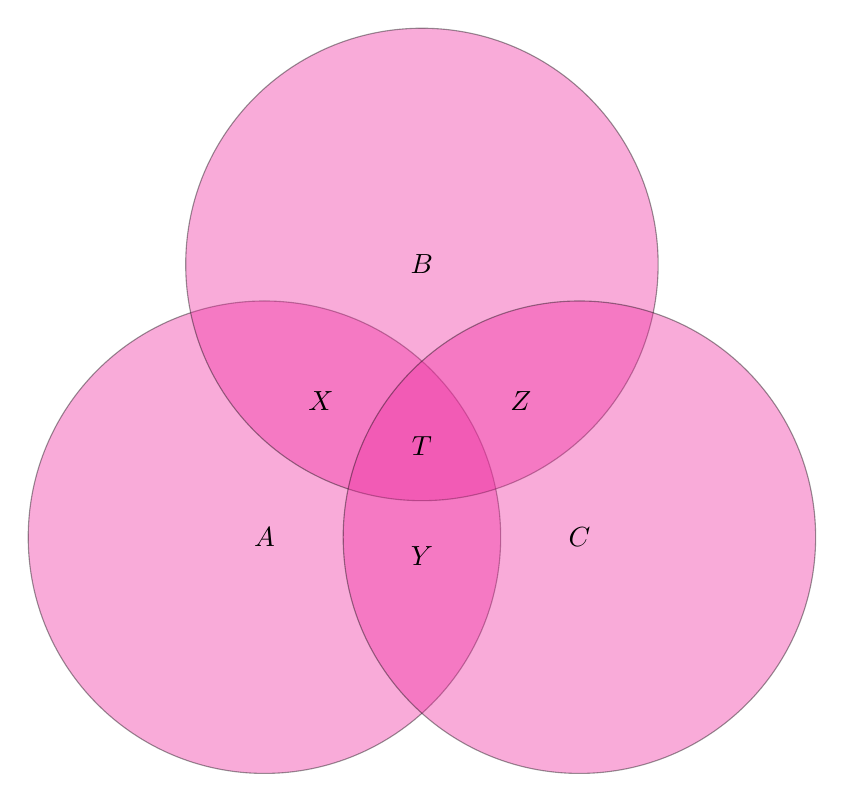
\begin{tikzpicture} [set/.style = {draw,
					    circle,
					    minimum size = 6cm,
					    fill=Rhodamine,
					    opacity = 0.4,
					    text opacity = 1}]
					 
					\node (A) [set] {$A$};
					\node (B) at (60:4cm) [set] {$B$};
					\node (C) at (0:4cm) [set] {$C$};
					 
					\node at (barycentric cs:A=1,B=1) [left] {$X$};
					\node at (barycentric cs:A=1,C=1) [below] {$Y$};
					\node at (barycentric cs:B=1,C=1) [right] {$Z$};
					\node at (barycentric cs:A=1,B=1,C=1) [] {$T$};
					 
				\end{tikzpicture}
		\section{Afsnit 2.1}
			\setcounter{subsection}{1}
			\subsection{2.1.2: Use set builder notation to give a description of each of these sets}
			\subsubsection{$\{0,3,6,9,12\}$}
					$3n|n\in\mathbb{N}$
				\subsubsection{$\{-3,-2,-1,0,1,2,3\}$}
					$n|n\in\mathbb{Z}$
			\setcounter{subsection}{6}
			\subsection{2.1.7: Determine whether each of these pairs of sets are equal.}
				\subsection{$\{1,3,3,3,5,5,5,5,5\},\{5,3,1\}$}
					Equal
				\subsection{$\{\{1\}\},\{1,\{1\}\}$}
					Not equal
				\subsection{$\emptyset, \{\emptyset\}$}
					Not equal, the right is not empty it contains the empty set
				\setcounter{subsection}{12}
				\subsection{2.1.13: Determine whether each of these statements is true or false}
					\subsubsection{$x\in\{x\}$}
						True
					\subsubsection{$\{x\}\subseteq \{x\}$}
						True
					\subsubsection{$\{x\}\in\{x\}$}
						False
					\subsubsection{$\{x\}\in\{\{x\}\}$}
						True
					\subsubsection{$\emptyset \subseteq \{x\}$}
						True
					\subsubsection{$\emptyset \in \{x\}$}
						False
				\setcounter{subsection}{20}
				\subsection{2.1.21: What is the cardinality of each of these sets?}
					\subsubsection{$\{a\}$}
						1
					\subsubsection{$\{\{a\}\}$}
						1
					\subsubsection{$\{a,\{a\}\}$}
						2
					\subsubsection{$\{a,\{a\},\{a,\{a\}\}\}$}
						3
				\setcounter{subsection}{22}
				\subsection{Find the power set of each of these sets, where $a$ and $b$ are distinct elements}
					\subsubsection{\{a\}}
						$P(a)=\{\{a\},\emptyset\}$
					\subsubsection{$\{a,b\}$}
						$P(b)=\{\{a\},\{b\},\emptyset, \{a,b\}\}\}$
					\subsubsection{$\{\emptyset,\{\emptyset\}\}$}
						$P(c)=\{\emptyset, \{\emptyset\},\{\emptyset,\{\emptyset\}\}\}$
		\chapter{Uge}
			\section{Afsnit 5.1}
				\setcounter{subsection}{22}
				\subsection{5.1.23: For which nonnegative integers $n$ is $2n + 3 \leq 2^n$ ? Prove your answer}
					\begin{align*}
						\forall n \in \mathbb{Z}^-: 0<2^n<1\\
						\forall n \in n<-1: n < 0
						\text{basis}: P(4)\\
						\text{Antagelse}: P(k):2\cdot k+3\leq 2^k\\
						\text{skridt}\\
						&=2(k+1)+3\\
						&=2k+3+2\\
						&\leq 2^k+2\\
						&\leq 2^k\cdot 2 \text{Da k >=1}\\
						&\leq 2^{k+1}\\
						2(k+1)&\leq 2^{k+1}
					\end{align*}
				\section{Løs følgende opgave fra et tidligere eksamenssæt:Hvilke af nedenstående mængder er lig med $A={2n+1|n\in \mathbb{Z}}$}
					\subsection{$S_1=\{1,2,4,8,...\}$}
						Falsk
					\subsection{$S_2=\{2,3,5,9,...\}$}
						Falsk
					\subsection{$S_3=\{1,3,5,7,...\}$}
						Falsk
					\subsection{$S_4=\{...,-3,-1,1,3,...\}$}
						Sandt
					\subsection{$S_5=\{n\in\mathbb{Z}|\exists k \in \mathbb{Z}: n=2k+1$}
						Sandt
					\subsection{$S_6=\{n\in\mathbb{Z}|\exists!k\in\mathbb{N}:n=2k+1\}$}
						Sandt
					\subsection{$S_7=\{n\in\mathbb{Z}|\forall k \in \mathbb{Z}: n\neq 2k\}$}
						Sandt
					\subsection{$S_8=\{n\in\mathbb{Z}|\exists k\in \mathbb{Z}:2n+1=k\}$}
						Falsk
			\setcounter{section}{0}
			\section{Afsnit 5.1}
				\setcounter{subsection}{77}
				\subsection{5.1.78 Construct a tiling using right triominoes of the $4 \times 4$ checkerboard with the square in the upper left corner removed}
					O b m m\\
					b b v m\\
					e v v n\\
					e e n n
				\subsection{5.1.79: Construct a tiling using right triominoes of the $8 \times 8$ checkerboard with the square in the upper left corner removed}
					Here the last tiling can be used and rotated so the new three versions missing cornors to construct a new tile.
				\subsection{Generaliser din løsning til opgave 78–79, så den virker for et skakbræt med $2^n\times 2^n$felter, for alle $n\in \mathbb{Z}^+$}
					Like described in 5.1.79 the previus tiling can be used and rotated so the holes will fill out a right triominoe which will complete the tiling.
			\section{Afsnit 2.2}
				\setcounter{subsection}{20}
				\subsection{2.2.21: Show that if $A$ and $B$ are sets then:}
					\subsubsection{$A-B=A\cup \overline{B}$}
						Fratrækkelsen af $B$ vil betyde at overlappet vil fjernes fra $A$. Dermed er det lig med den anden side, da alt i $A$ bliver beholdt som ikke overlapper $B$.
					\subsubsection{$(A\cup B)\cap (A\cup \overline{B})=A$}
						Da mængden $A$ bliver forenet med både $B$ og $\overline{B}$ og hver bliver taget fra hinanden vil det eneste tilbage være $A$
				\setcounter{subsection}{30}
				\subsection{2.2.31: What can you say about the sets A and B if we know that}
					\subsubsection{$A\cup B=A$}
						$B=\emptyset \lor B=A$ 	
					\subsubsection{$A\cap B=A$}
						$A=B$
					\subsubsection{$A-B=A$}
						$B=\emptyset \lor B\cap A = \emptyset$
					\subsubsection{$A\cap B=B\cap A$}
						Nothing that is just the complimentary law.
					\subsubsection{$A-B=B-A$}
						$A=B \lor A=\emptyset \land B=\emptyset$
			\setcounter{section}{0}
			\section{Afsnit 2.2}
				\setcounter{subsection}{24}
				\subsection{2.2.25: Prove the first distributive law from Table 1 by showingthat if $A$, $B$, and $C$ are sets, then $A \cup (B \cap C) = (A\cup B) \cap (A \cup C)$.}
					\begin{center}
						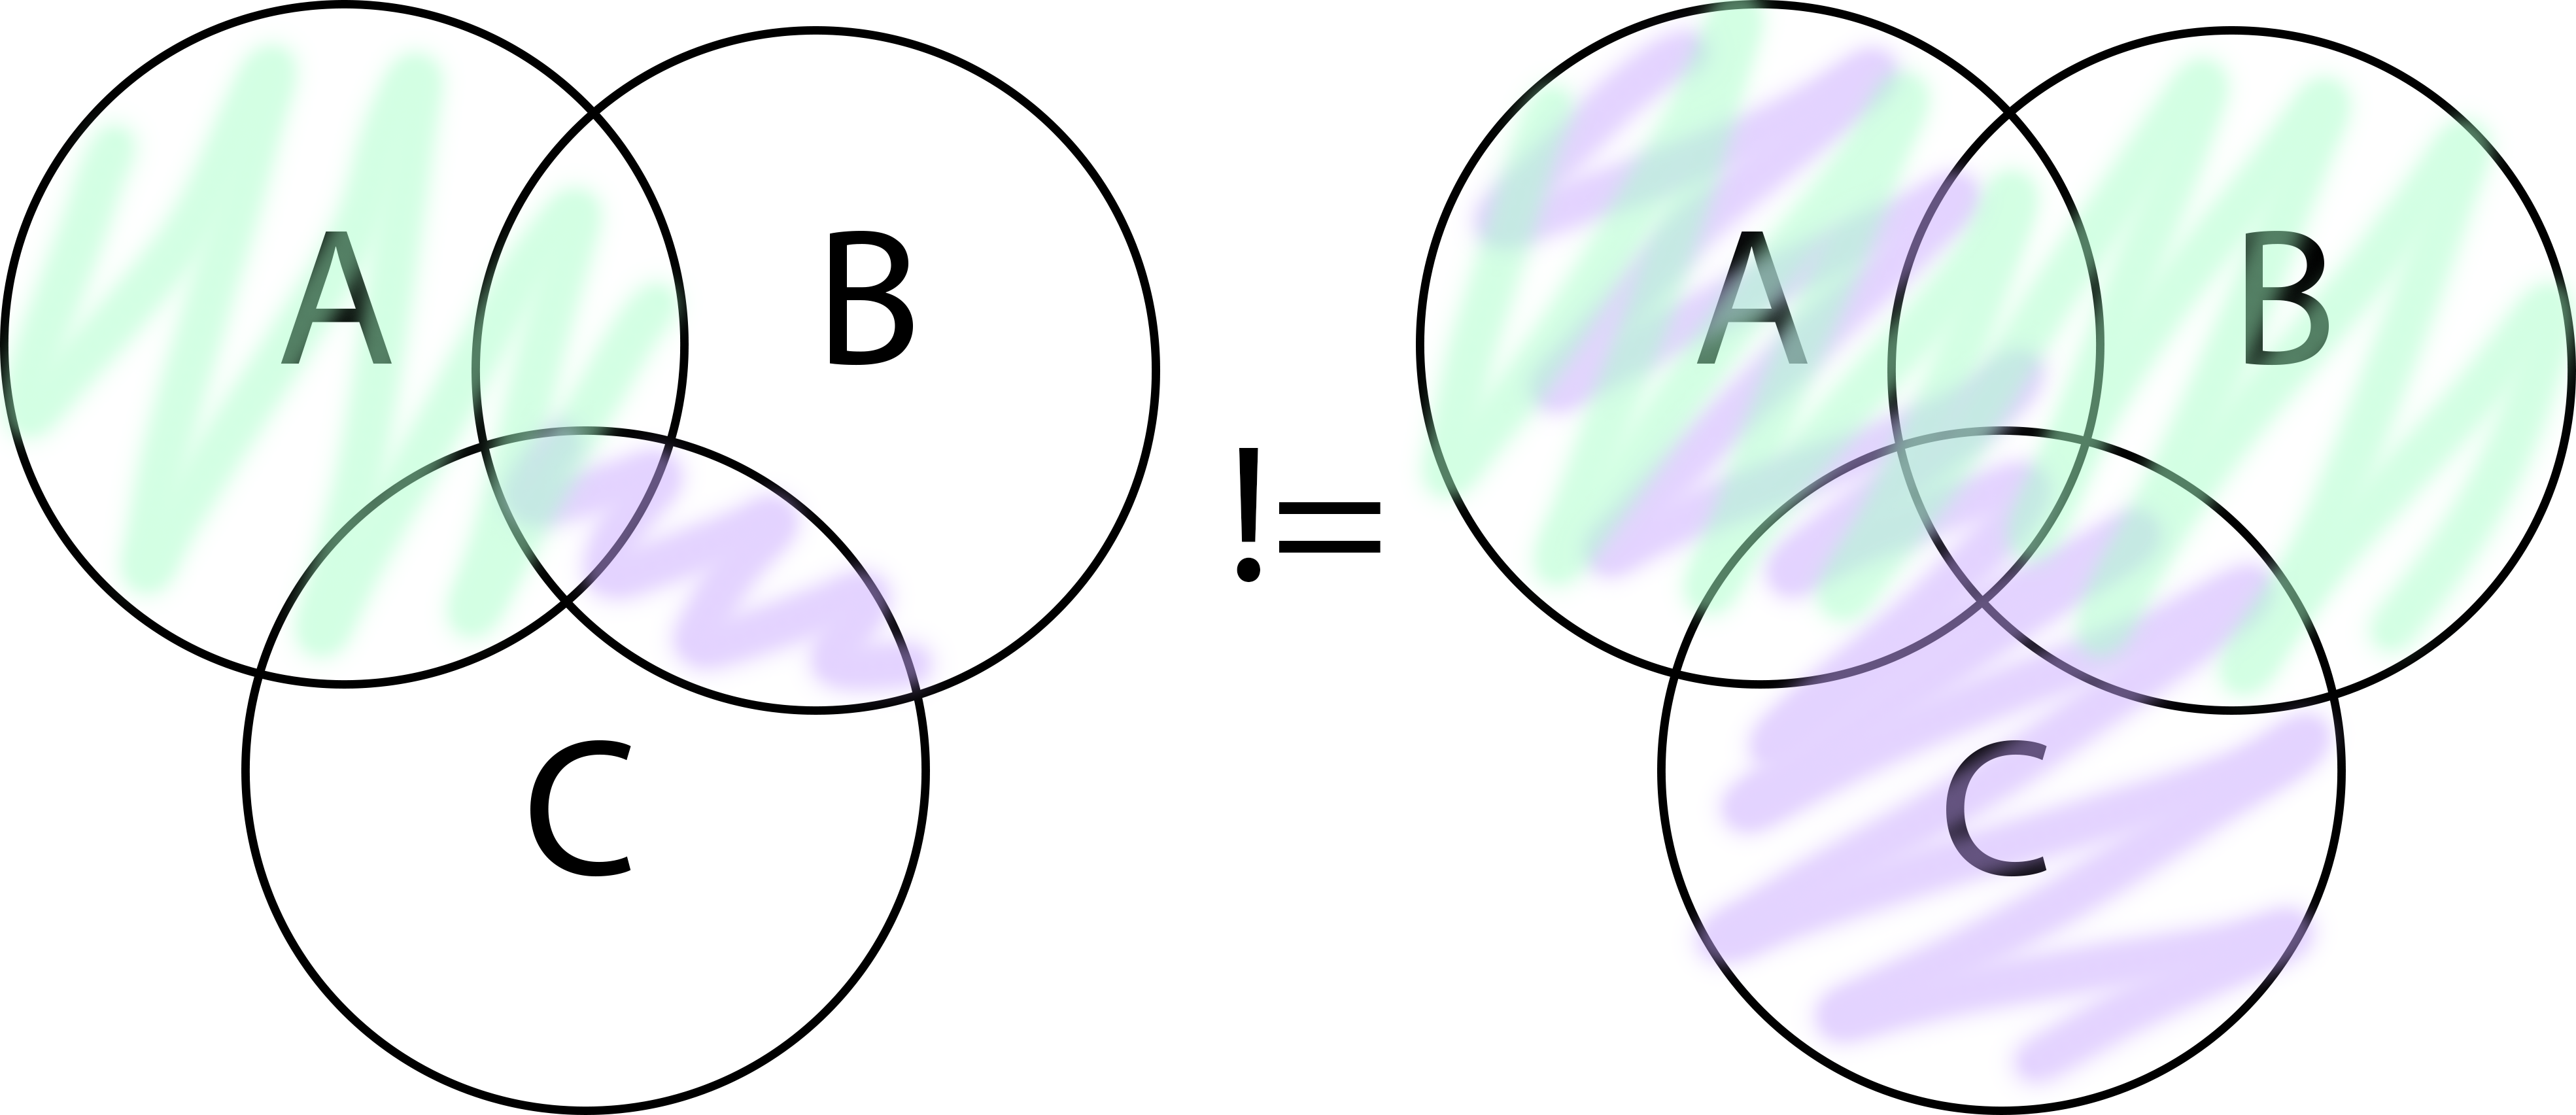
\includegraphics[width=250px]{assets/2.25.png}
					\end{center}
				Det samlet areal på venstre og det kun grønne på højre og de er ikke ens.
			\section{Løs følgende opgave fra et tidligere eksamenssæt: Betragt de to mængder $S_1=(A-C)\cup (B\cap C)$ og $S_2=(A\cup C) -(\overline{B}\cap C)$. Afgør om $S_1=S_2$}
				\begin{center}
					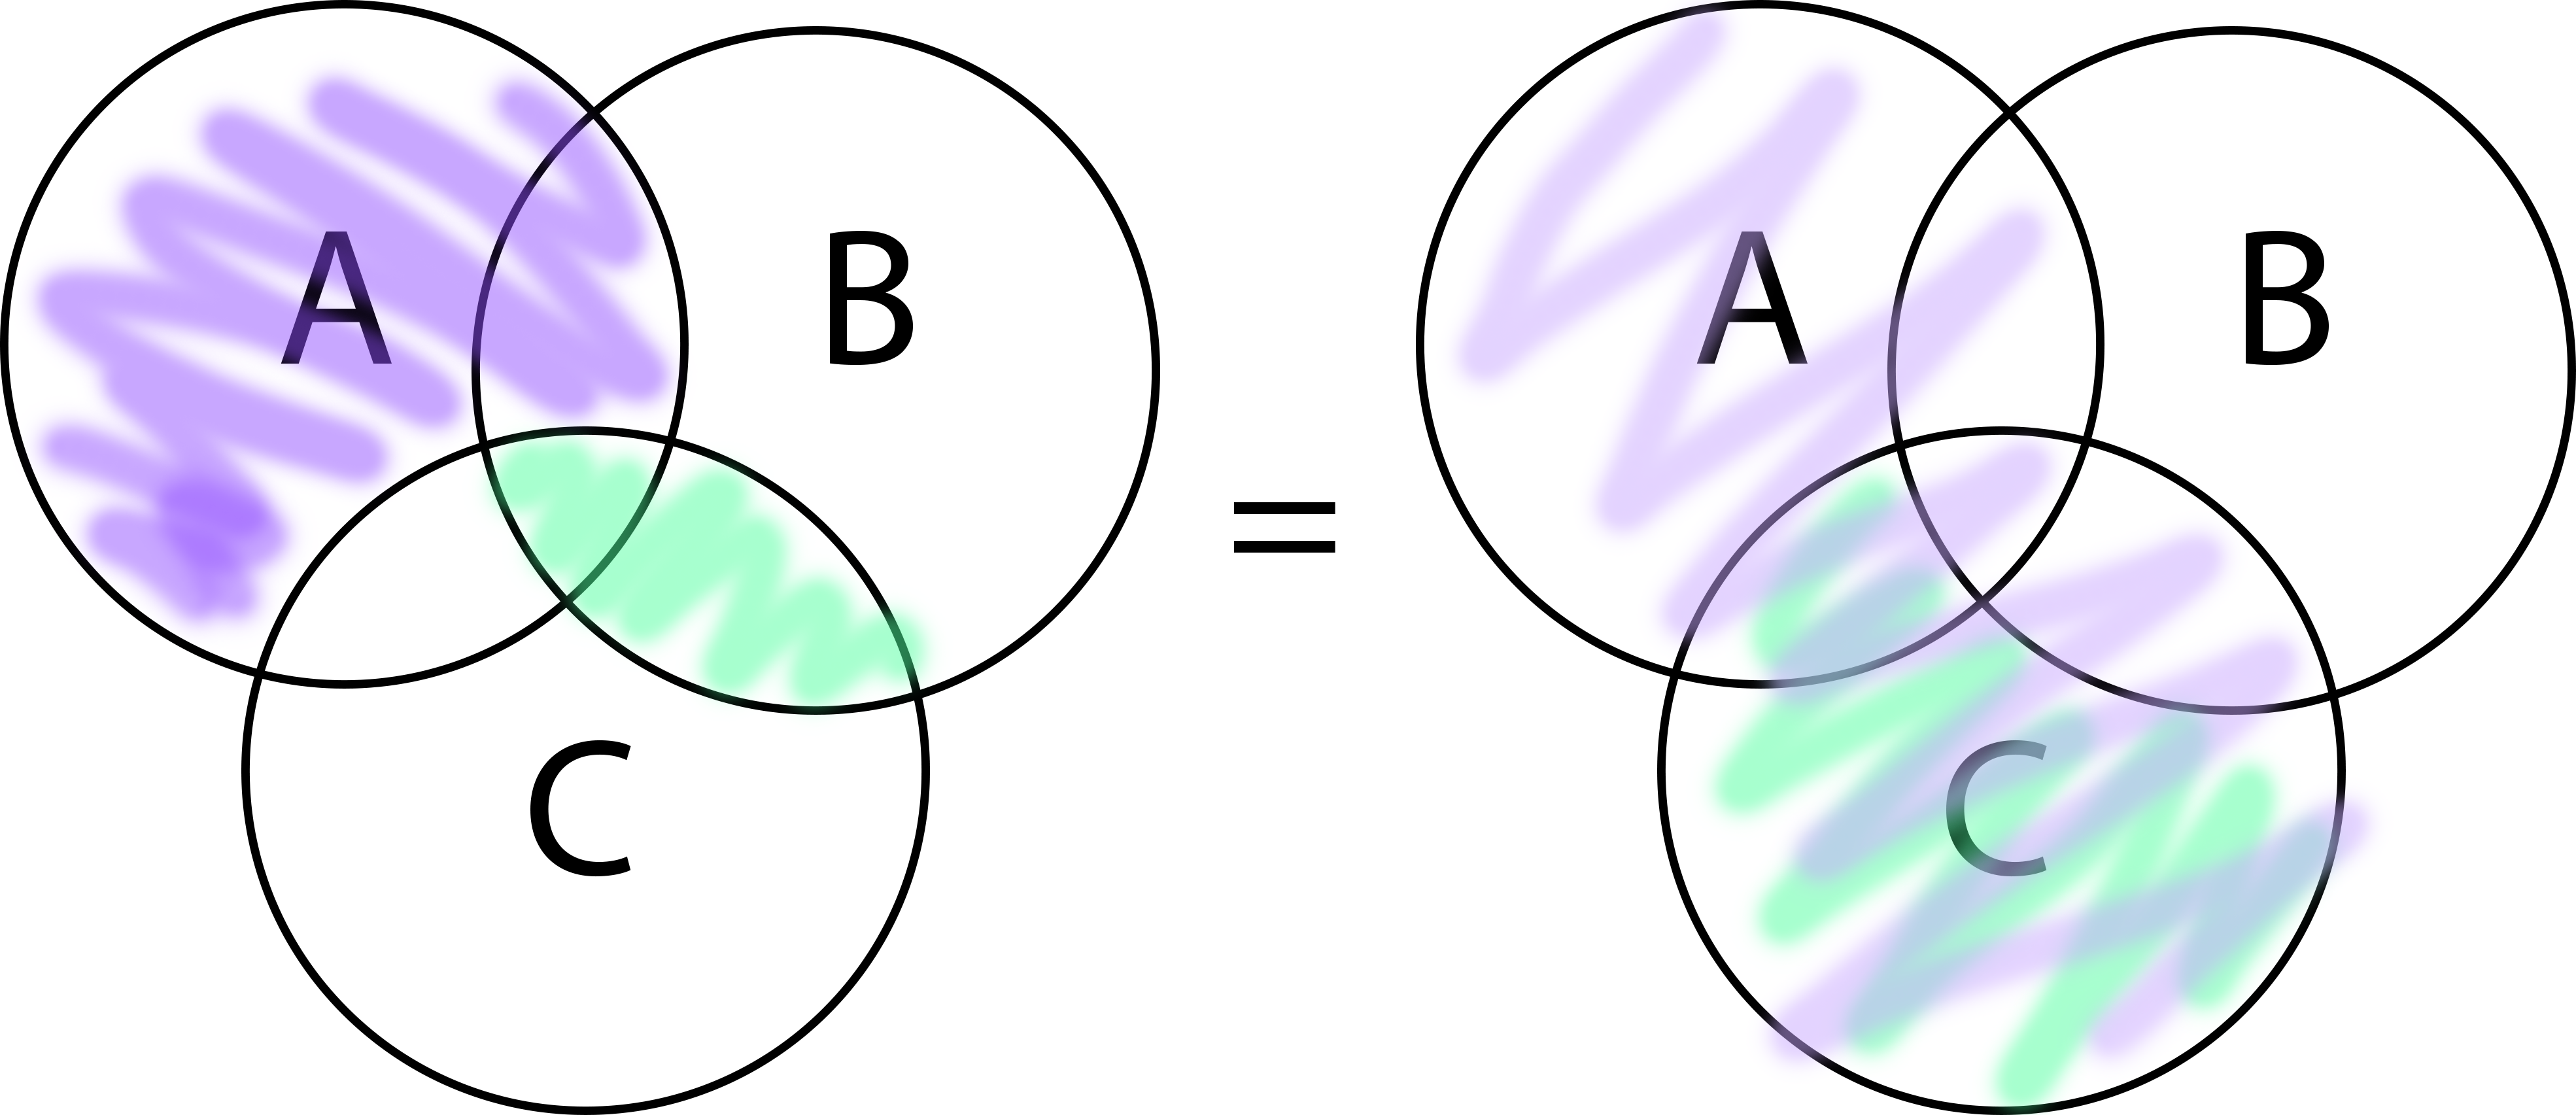
\includegraphics[width=250px]{assets/2.26.png}
				\end{center}
				Det samlet areal på venstre og det kun lilla på højre. Dermed ens.
			\setcounter{section}{0}
			\section{Afsnit 2.3}
				\setcounter{subsection}{0}
				\subsection{2.3.1: Why is $f$ not a function from $\mathbb{R}$ to $\mathbb{R}$ if}
					\subsubsection{$f(x)=\frac{1}{x}$?}
						$x$ can not be 0.
					\subsubsection{$f(x)=\sqrt{x}$?}
						$x$ can only be positive values
					\subsubsection{$f(x)=\pm\sqrt{x^2+1}$?}
						No value between -1 and 1
				\setcounter{subsection}{8}
				\subsection{2.3.9: Find these values.}
					\subsubsection{$\lceil \frac{3}{4}\rceil$}
						1
					\subsubsection{$\lfloor 1.1 \rfloor$}
						2
					\subsubsection{$\lfloor -0.1 \rfloor$}
						-1
					\subsubsection{$\lceil -0.1 \rceil$}
						0
				\setcounter{subsection}{11}
				\subsection{2.3.12: Determine whether each of these functions from $\mathbb{Z}$ to $\mathbb{Z}$ is one-to-one.}
					\subsubsection{$f(n)=n-1$}
						1-2-1
					\subsubsection{$f(n)=n^2+1$}
						Not 1-2-1 because negativ values map to the same as possitive with some offset
				\subsection{2.3.13: Which functions in Exercise 12 are onto?}
					\subsubsection{$f(n)=n-1$}
						yes
					\subsubsection{$f(n)=n^2+1$}
						Not 0 or negative values
				\subsection{ Which functions in Exercise 12 are bijektiv?}
					\subsubsection{$f(n)=n-1$}
						yes
					\subsubsection{$f(n)=n^2+1$}
						No
				\setcounter{subsection}{37}
				\subsection{2.3.38: Find $f \cdot g$ and $g\cdot f$ , where $f (x) = x^2 + 1$ and $g(x) = x + 2$, are functions from $\mathbb{R}$ to $\mathbb{R}$}
					$f\cdot g = f(x+2) = (x+2)^2+1=x^2+4x+4$\\
					$g\cdot f=g(x^2+2)=x^2+4$
				\subsection{2.3.39: Find $f + g$ and $fg$ for the functions $f$ and $g$ given in Exercise 38}
					$f+g=x^2+3+x$\\
					$fg=(x^2+1)(x+2)=x^3+2x^2+x+2$	
				\subsection{2.3.40: Let $f(x) = ax + b$ and $g(x) = cx + d$, where $a, b, c$, and $d$ are constants. Determine necessary and sufficient conditions on the constants $a, b, c$, and $d$ so that $f\cdot g = g\cdot f$ .}
					All constants can be zero
				\subsection{2.3.41: Show that the function $f(x) = ax + b$ from $\mathbb{R}$ to $\mathbb{R}$, where $a$ and $b$ are constants with $a \neq 0$ is invertible, and find the inverse of $f$ .}
					$y=ax+b$\\
					$\frac{y}{a}-b=x$
		\chapter{Uge}
			\section{Afsnit 2.3}
				\setcounter{subsection}{8}
				\subsection{2.3.9: Find these values}
					\setcounter{subsubsection}{4}
					\subsubsection{$\lceil 3 \rceil$}
						3
					\subsubsection{$\lfloor -1 \rfloor$}
						-1
					\subsubsection{$\lfloor \frac{1}{2}+\lceil \frac{3}{2}\rceil\rfloor$}
						2
					\subsubsection{$\lfloor \frac{1}{2}\cdot \lfloor\frac{5}{2}\rfloor\rfloor$}
						1
				\setcounter{subsection}{11}
				\subsection{2.3.12: Determine whether each of these functions from $\mathbb{Z}$ to $\mathbb{Z}$ is one-to-one (surjektiv)}
					\setcounter{subsubsection}{2}
					\subsubsection{$f(n)=n^3$}
						No
					\subsubsection{$f(n)=\lceil \frac{n}{2}\rceil$}
						Yes
					\subsection{2.3.13: Which functions in Exercise 12 are onto (injektiv)?}
					\setcounter{subsubsection}{2}
					\subsubsection{$f(n)=n^3$}
						Yes because $\sqrt[3]{\mathbb{Z}}=\mathbb{Z}$ has only one solution
					\subsubsection{$f(n)=\lceil \frac{n}{2}\rceil$}
						No because $f(3)=f(4)$
				\subsection{Hvilke af funktionerne i opgave 12 c–d er bijektive?}
					None
				\setcounter{subsection}{70}
				\subsection{Find the inverse function of $f(x)=x^3+1$.}
					$x=\sqrt[3]{y-1i}$
			\section{Afsnit 2.5}
				\setcounter{subsection}{1}
				\subsection{2.5.2: Determine whether each of these sets is finite, countably infinite, or uncountable. For those that are countably infinite, exhibit a one-to-one correspondence between the set of positive integers and that set}
					\subsubsection{the intergers greater than 10}
						countably infinite
					\setcounter{subsubsection}{2}
					\subsubsection{the integers with absolute value less than 1,000,000}
						finite
					\setcounter{subsubsection}{4}
					\subsubsection{the set $A\times\mathbb{Z}^+$ where $A={2,3}$}
						countably infinite
				\setcounter{subsection}{15}
				\subsection{2.5.16: Show that a subset of a countable set is also countable}
					For a set the subset is defined as being atleast the emptyset og contain elements from the countable set. Due to the empty set being countable and the set being countable everything between must also be countable.
				\setcounter{subsection}{14}
				\subsection{2.5.15: Show that if $A$ and $B$ are sets, $A$ is uncountable and $A\subseteq B$ then $B$ is uncountable.}
					Since the subset is uncountable it means that the set contains more than or equal amounts of elements which is uncountable.\\
			\section{Afsnit 5.3}
				\setcounter{subsection}{0}
				\subsection{5.3.1: Find $f(1),f(2),f(3)$ and $f(4)$ if $f(n)$ is deifned recursively by $f(0)=1$ and for $n=0,1,2,...$}
					\subsubsection{$f(n+1)=f(n)+2$}
						\begin{align*}
							f(0)=1\\
							f(1)=3\\
							f(2)=5\\
							f(3)=7\\
							f(4)=9
						\end{align*}
					\subsubsection{$f(n+1)=3f(n)$}
						\begin{align*}
							f(0)=1\\
							f(1)=3\\
							f(2)=9\\
							f(3)=27\\
							f(4)=81
						\end{align*}
				\setcounter{subsection}{6}
				\subsection{5.3.7: Give a recursive definition of the sequence $\{a_n\},n=1,2,3,...$ if }
					\subsubsection{$a_n=6n$}
						$f(0)=0$\\
						$f(n+1)=f(n)+6$
					\subsubsection{$a_n=2n+1$}
						$f(0)=1$\\
						$f(n+1)=f(n)+2$
			\section{Afsnit 2.5}
				\setcounter{subsection}{24}
				\subsection{2.5.25: Prove that if it is possible to label each element of an ininite set S with a finite string of keyboard characters, from a finite list characters, where no two elements of S have the same label, then S is a countably infinite set.}
					By assigning every digit to a the corresponding charachter from the alphabet every number can be can be converted to a string. Here can negatives be represented by y or just any charachter which is not in use. \\
					Then any charachter from $\mathbb{Z}$ will be represented by a finite string.\\
				\subsection{2.5.26:Use Exercise 25 to provide a proof different from that in the text that the set of rational numbers is countable. [Hint: Show that you can express a rational number as a string of digits with a slash and possibly a minus sign.]}
					Since a rational number is $\mathbb{Z}/\mathbb{Z}$ means represented as a string it simply contains two finite string and a charachter representing a slash.
				\subsection{2.5.27: Show that the union of a countable number of countable sets is countable}
					By given all alements an index, the sum of all indexes from the given sets will not exceed infinite but stay finite.
		\chapter{Uge}
			\section{Afsnit 2.5}
				\setcounter{subsection}{1}
				\subsection{2.5.2: Determine whether each of these sets is finite, countably infinite, or uncountable. For those that are countably infinite, exhibit a one-to-one correspondence between the set of positive integers and that set.}
					\setcounter{subsubsection}{1}
					\subsubsection{The odd negative integers}
						Countably infinite
					\setcounter{subsubsection}{3}
					\subsubsection{The real numbers between 0 and 2}
						Countably infinite
					\setcounter{subsubsection}{5}
					\subsubsection{The integers that are multiples of 10}
						Countably infinite
				\setcounter{subsection}{27}
				\subsection{Show that the set $\mathbb{Z}^+\times \mathbb{Z}^+$ is countable}
					Like the proof for the set $Q=\frac{a}{b}|a,b \in Z$, where instead of a division its just a combination of numers in a tuble. \\
			\section{Afsnit 5.3}
				\setcounter{subsection}{0}
				\subsection{5.3.1 Find $f(1),f(2),f(3), and f(4)$ if $f(n)$ is defined recursively for $f(0)=1$ and for $n=0,1,2,...$}
					\setcounter{subsubsection}{2}
					\subsubsection{$f(n+1)=2^{f(n)}$}\
						\begin{align*}
							f(0)=1\\
							f(1)=2\\
							f(2)=4\\
							f(3)=16\\
							f(4)=65536
						\end{align*}
					\subsubsection{$f(n+1)=f(n)^2+f(n)+1$}
						\begin{align*}
							f(0)=1\\
							f(1)=3\\
							f(2)=13\\
							f(3)=183\\
							f(4)=33673
						\end{align*}
				\setcounter{subsection}{6}
				\subsection{5.3.7 Give a recursive definition of the sequence ${a_n},n=1,2,3,...$ if }
					\setcounter{subsubsection}{2}
					\subsubsection{$a_n=10^n$}
						\begin{align*}
							f(0)=1;
							f(n+1)=n*10
						\end{align*}
					\subsubsection{$a_n=5$}
						\begin{align*}
							f(0)=5\\
							f(n+1)=f(n)
						\end{align*}
			\section{Bevis, at alle heltal $n\geq 8$ kan skrives som en sum af 3-taller og5-taller. Findes der et heltalk, sådan at alle heltal $n\leq k$ kan skrives som en sum af 4-taller og 5-taller?}
				basis\\ 
				$5\cdot 1 +3\cdot 1 = 8$\\
				$5\cdot 0 + 3\cdot 3 = 9$\\
				$5\cdot 2 + 3\cdot 0 = 10$\\
				Antagelse\\
				$f(n+3)=f(n)+3$\\
				Bevis\\
				Som det kan ses med antagelse i de 2 basis vil $f(n-2)+3=f(n+1)$ man kunne den næste værdived at ligge 3 til og dermed kan samtlige tal findes på det grundlag.
			\section{Hvad er der galt med følgende bevis?}
				\textbf{Påstand}: Alle naturlige tal $n$ er lige.\\
				\textbf{Bevis}: ved stærk induktion over $n$\\
				Basis: 0 er et lige tal.\\
				\emph{Induktionsantagelse}: Ethvert naturligt tal $m<k$ er lige. D.v.s $m=2l$, hvor $l\in \mathbb{Z}$\\
				\emph{Induktionsskridt}:\\
				\begin{align*}
					k-2&=2l&&\text{hvor }\: l\in\mathbb{Z}\\
					k&=2l+2&&\text{hvor}\: l\in\mathbb{Z}\\
					k&=2(l+1)&&\text{hvor}\: l+1\in\mathbb{Z}
				\end{align*}
				Problemet ligger i at beviset er ikke er stærk induktion, da der kun er 1 basis og beviset ikke er induktion. Der udføres ikke induktion, da antagelsen siger at ethvert tal mindre end $k$ som er defineret som 2 gange et naturligt tal. Hvor at det så bliver vist at $k=2(l+1)$. Dermed bliver det bevist at for et naturligt tal multipliceret med 2 er mindre en det samme tal multipliceret med 2 plus 1.
			\setcounter{section}{0}
			\section{Betragt følgen $\{a_n\}$ defineret ved $$a_n=\begin{cases}n,&\text{hvis}\; 1\leq n \leq 2\\ a_{n-1}+2a_{n-2},&\text{hvis}\; n\geq 3\end{cases}$$ bevis vha. induktion at $a_n=2^{n-1}$,for alle $n\geq 1$.}
				basis\\
				$a_1 = 2^{1-1}=1$\\
				$a_2 = 2^{2-1}=2$\\
				Antagelse\\
				$a_{k-1}+2a_{k-2}=2^{k-1}$\\
				Induktionsskridt\\
				\begin{align*}
					a_{k-1}+2a_{k-2}=2^{k-1}\\[4mm]
					a_k+2a_{k-1}=2^k\\
					2^{k-1}+2a_{k-1}=2^k\\
					2a_{k-1}=2^k-2^{k-1}\\
					2a_{k-1}=2^{k-1}\\
					a_{k-1}=2^{k-2}\\
					a_k=2^{k-1}
				\end{align*}
				dermed $a_n->a_{n+2}$
			\section{Afsnit 5.2}
				\setcounter{subsection}{9}
				\subsection{2.5.10: Give an example of two uncountable sets $A$ and $B$ such that $A-B$ is}
					\subsubsection{Finite}
						$A=\{1,2\}$\\
						$B=\{2\}$
					\subsubsection{Countably infinite}
						$A=\{a\in Z\}$\\
						$B=\{1\}$
					\subsubsection{uncountable}
						$A=\{a\in R\}$\\
						$B\{1\}$
					
				\setcounter{subsection}{24}
				\subsection{Suppose that $P(n)$ is a propositinal function. Determinde for which positive integers $n$ the statement $P(n)$ must be true and justify your answer if}
					\subsubsection{$P(1)$ is true; for all positive integers $n$, if $P(n)$ is true, then $P(n+2)$ is true.}
						This is not true due to missing basis.
					\subsubsection{$P(1)$ and $P(2)$ are true; for all positive integers $n$ if $P(n)$ and $P(n+1)$ are true then $P(n+2)$ is true}
						True
					\subsubsection{$P(1)$ is true; for all positive integers $n$ if $P(n)$ is true, then $P(2n)$ is true.}
						No this will not tile alle positive integers
					\subsubsection{$P(1)$ is true; for all positive integers $n$ if $P(n)$ is true then $P(n+1)$ is true.}
						True
			\section{Afsnit 9.1}
				\setcounter{subsection}{0}
				\subsection{9.1.1 List the ordered paris in the relation $R$ from $A=\{0,1,2,3,4\}$ to $b=\{0,1,2,3\}$, where $(a,b)\in R$ if and only if}
					\subsubsection{a=b}
						$(a,b)|a\in A \land b \in B \land a=b$\\
						$\{(0,0),(1,1),(2,2),(3,3,)\}$
				\setcounter{subsection}{2}
				\subsection{9.1.3 For each of these relations on the set $\{1,2,3,4\}$, decide wheter it is reflexive, symmetric, antisymmetric or transitive}
					\subsubsection{$\{(2,2),(2,3),(2,4),(3,2),(3,3),(3,4)\}$}
						Transitive\\
						Not reflexive due to missing $(1,1),(4,4)$\\
						Not symmetric due to missing $(4,2),(4,3)$\\
						Not antisymmetric due to having $(2,3),(3,2)$
				\setcounter{subsection}{6}
				\subsection{9.1.7 Determinde wheter the relation $R$ on the set of all integers os reflexive, symmetric, antisymmetric, and/or transitive, where $(x,y)\in R$ if and only if}
					\subsubsection{$x\neq y$}
						Not reflexive, symmetric, not antisymmetric, transitive
				\setcounter{subsection}{31}
				\subsection{9.1.32 Let $R$ be the relation $\{(1,2),(1,3),(2,3),(2,4),(3,1)\}$, and let $S$ be the relation $\{(2,1),(3,1),(3,2),(4,2)\}$. Find $R \circ S$?}
					$\{(2,2),(3,2),(2,3),(3,3),(3,4),(4,4)\}$\\[5mm]
				$R_1=\{(a,b)\in R^2|a>b\}$\\
				$R_2=\{(a,b)\in R^2|a\geq b\}$\\
				$R_3=\{(a,b)\in R^2|a<b\}$\\
				$R_4=\{(a,b)\in R^2 | a\leq b\}$\\
				$R_5=\{(a,b)\in R^2|a=b\}$\\
				$R_6=\{(a,b)\in R^2|a\neq b\}$
				\setcounter{subsection}{35}
				\subsection{9.1.36 Find}
					\subsubsection{$R_1\circ R_1$}
						$R_1\circ R_1 = \{(a,b)\in R^2|a\geq c | c>b\}$
					\subsubsection{$R_1\circ R_2$}
						$R_1\circ R_2 = \{(a,b)\in R^2|a>b\}$
					\subsubsection{$R_1 \circ R_6$}
						$R_1\circ R_6 = \{(a,b)\in R^2|a>b$
					\subsubsection{$R_3\cap R_5$}
						$R_3\cap R_5 = \emptyset$
				\setcounter{subsection}{33}
				\subsection{9.1.34: Find}
					\subsubsection{$R_1\cup R_3$}
						$R_1\cup R_3 = R_6$
					\setcounter{subsubsection}{2}
					\subsubsection{$R_2\cap R_4$}
						$R_2\cap R_4=(a,b)\in R^2$
					\setcounter{subsubsection}{4}
					\subsubsection{$R_1-R_2$}
						$R_1-R_2=\emptyset$
					\setcounter{subsubsection}{7}
					\subsubsection{$R_2\oplus R_4$}
						$R_2\oplus R_4 = \{(a,b)\in R^2|\neq(a\neq b)\}$
			\setcounter{section}{0}
			\section{Afsnit 9.1}
				\setcounter{subsection}{0}
				\subsection{9.1.1.b: List the ordered pairs in the relation $R$ from $A=\{0,1,2,3,4\}$ to $B=\{0,1,2,3\}$, where $(a,b)\in R$ if and only if $a+b=4$}
					$\{(0,4),(1,3),(3,1),(2,2)\}$
				\setcounter{subsection}{6}
				\subsection{9.1.7.f Determinde whether the relation $R$ on the set of all integers is reflexive, symmetric, antisymmetric, and/or transitive, where $(x,y)\in R$ if and only if $x$ and $y$ are both negative}
					The relation is reflexive, symmetric and transitive
				\setcounter{subsection}{31}
				\subsection{9.1.32: Let $R$ be the relation $\{(1,2),(1,3),(2,3),(2,4),(3,1)\}$, and let $S$ be the relation $\{(2,1),(3,1),(3,2),(4,2)\}$. Find $S\circ R$.}
					$S\circ R=\{(1,1),(1,2),(2,2),(2,1)\}$
				\subsection{9.1.33: Let $R$ be hte reltion on the set of people consiting of pairs $(a,b)$, where $A$ is a prent of $b$. Let $S$ be the relation on hte set of people consisting of pairs $(a,b)$, where $a$ and $b$ are siblings (brother and sisters). Wat are $S \circ R$ and $R\circ S$}
					$R\circ S$ will give all the parents to their corresponding daughter/son\\
					$S\circ R$ Will be empty
				\setcounter{subsection}{51}
				\subsection{Suppose that $R$ and $S$ are reflexive relations on a set $A$. Prove or disprove each of these statements}
					\subsubsection{$R\cup S$ is reflexive}
						True
					\subsubsection{$R\cap S$ is reflexive}
						True
					\subsubsection{$R\oplus S$ is irreflexive}
						True
					\subsubsection{$R-S$ is irreflexive}
						True
					\subsubsection{$S\circ R$ is reflexive}
						True if $S\circ R \neq \emptyset$
			\section{Afsnit 9.3}
				\setcounter{subsection}{0}
				\subsection{9.3.1.f: Represent each of these relations on $\{1,2,3\}$ with a matrix (with the lements of this set listed in increasing order). $\{(1,2),(2,1),(2,2),(3,3)\}$}
					\begin{table}[h!]
						\begin{tabular}{|l|l|l|}
						\hline
						0 & 1 & 0 \\ \hline
						1 & 1 & 0 \\ \hline
						0 & 0 & 1 \\ \hline
						\end{tabular}
					\end{table}
				\setcounter{subsection}{17}
				\subsection{9.3.18.b: Draw the direted graphs representing each of the relations from Exercise 1}
					$\{(1,2),(2,1),(2,2),(3,3)\}$\\
					\begin{tikzpicture}[scale=3]
						\tikzstyle{vertex}=[circle,draw=black]
						\node[vertex](v1) at (0,0.75) {1};
						\node[vertex](v2) at (1,0.75) {2};
						\node[vertex](v3) at (0.5,0) {3};
						\draw[blue, ->,transform canvas={xshift=0pt,yshift=2.5pt}](v1) -- (v2);
						\draw[blue, <-,transform canvas={xshift=0pt,yshift=-2.5pt}](v1) -- (v2);
						\path(v2) edge [loop above, color=blue] node {}(v2);
						\path(v3) edge [loop above, color=blue] node {}(v3);
					\end{tikzpicture}	
				\setcounter{subsection}{30}
				\subsection{9.3.31 Determinde whether the relations represented by the directed graphs shown in Exercises 23-25 are reflexive, irreflexive, symmetric, antisymmetric and/or transitive}
					26\\
					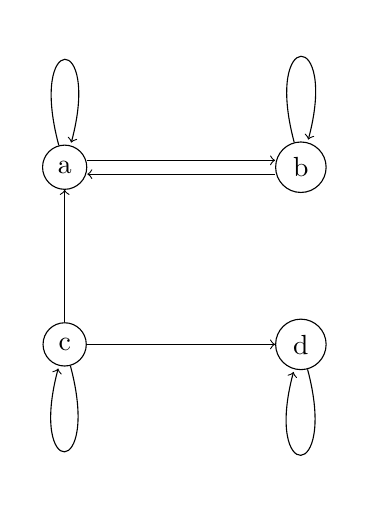
\begin{tikzpicture}[scale=3]
						\tikzstyle{vertex}=[circle,draw=black]
						\node[vertex](v1) at (0,0.75) {a};
						\node[vertex](v2) at (1,0.75) {b};
						\node[vertex](v3) at (0,0) {c};
						\node[vertex](v4) at (1,0) {d};
						\draw[ ->,transform canvas={xshift=0pt,yshift=2.5pt}](v1) -- (v2);
						\draw[ <-,transform canvas={xshift=0pt,yshift=-2.5pt}](v1) -- (v2);
						\draw[->](v3) -- (v1);
						\draw[->](v3) -- (v4);
						\path(v1) edge [loop above] node {}(v1);
						\path(v2) edge [loop above] node {}(v2);
						\path(v3) edge [loop below] node {}(v3);
						\path(v4) edge [loop below] node {}(v4);
					\end{tikzpicture}\\
					27\\
					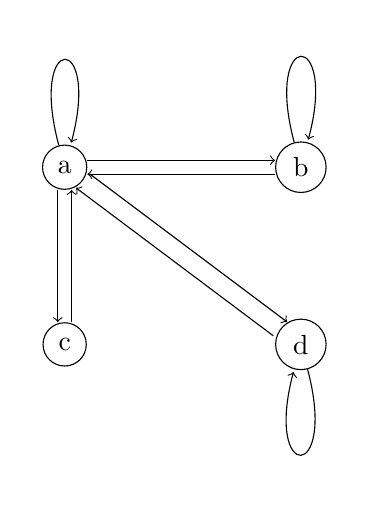
\begin{tikzpicture}[scale=3]
						\tikzstyle{vertex}=[circle,draw=black]
						\node[vertex](v1) at (0,0.75) {a};
						\node[vertex](v2) at (1,0.75) {b};
						\node[vertex](v3) at (0,0) {c};
						\node[vertex](v4) at (1,0) {d};
						\draw[ ->,transform canvas={xshift=0pt,yshift=2.5pt}](v1) -- (v2);
						\draw[ <-,transform canvas={xshift=0pt,yshift=-2.5pt}](v1) -- (v2);
						\draw[ ->,transform canvas={xshift=-2.5pt,yshift=0pt}](v1) -- (v3);
						\draw[ <-,transform canvas={xshift=2.5pt,yshift=0pt}](v1) -- (v3);
						\draw[ ->,transform canvas={xshift=2.5pt,yshift=2.5pt}](v1) -- (v4);
						\draw[ <-,transform canvas={xshift=-2.5pt,yshift=-2.5pt}](v1) -- (v4);
						\path(v1) edge [loop above] node {}(v1);
						\path(v2) edge [loop above] node {}(v2);
						\path(v4) edge [loop below] node {}(v4);
					\end{tikzpicture}\\
					26 is reflexive\\
					27 is irreflexive,symmetric, transitive
			\section{Afsnit 9.1}
				\setcounter{subsection}{56}
				\subsection{9.1.57: Let $R$ be a relation that is reflexive and transitive. Prove that $R^n=R$ for all positve integers $n$}
					The relation $R$ can be described as $R=\{(a,b)\in R|a\geq b\}$\\
					It can then here be seen that for any two numbers $a\geq b $ the lowest posiible positive intger is $a^1 \geq b^1$ which is true. From there it can be seen that from when n is greater than 1 it will still be true.
				\setcounter{subsection}{60}
				\subsection{Suppose that the relation $R$ is irreflexive. Is $R^2$ necessarily irreflexive? Give a reason for your answer}
					No, if the definition set is in the negative and positive integers, $R$ could contain $(-1,1)$ which when squared will be $(1,1)$ therefore making it not irreflexive.
			\section{Afsnit 9.3}
				\setcounter{subsection}{8}
				\subsection{9.3.9: How many nonzero entries does the matrix representing the relation $R$ on $A=\{1,2,3,...,100\}$ consisting of the first 100 positive integers have if $R$ is}
					\subsubsection{$\{(a,b)|a>b\}$?}
						$100\cdot 100 /2-100=4900$
					\setcounter{subsubsection}{2}
					\subsubsection{$\{(a,b)|a=b+1\}$?}
						$100\cdot 100 /2-100=4900$
			\section{Betragt følgende binære relation på $\mathbb{N}$}
			$$R=\{(a,b)|a\cdot b\leq a+b\}$$
				\subsection{Angiv samtlige elementer i $R$}
					$R=\{1,a)|a\in \mathbb{N}\}$
				\subsection{Er $R$ symmetrisk}
					Ja, i en matrice vil række 1 hver den eneste udfyldt  både horizontal og vertikalt.\\
				\subsection{Hvad er kardinaliteten af $R$}
					$|R|=\aleph_0$
			\setcounter{section}{0}
			\section{Afsnit 9.4}				
				\setcounter{subsection}{0}
				\subsection{9.4.1: Let $R$ be the relation on the set $\{0,1,2,3\}$ containing the ordered pairs $(0,1),(1,1),(1,2),(2,0),(2,2),$ and $(3,0)$. Find the}
					\subsubsection{Reflexive closure of $R$}
						$r(R)=\{(0,0),(3,3)\}$
					\subsubsection{Symmetric closure of $R$}
						$s(R)=\{(1,0),(2,1),(0,2)\}$
			\section{Find den transitive lukning af relationen $R=\{(1,1),(2,3),(3,4),(3,5),(5,1)\}$.}
				$t(R)=\{(2,4),(2,5),(2,1),(3,1)\}$
			\section{Afsnit 9.5}
				\setcounter{subsection}{0}
				\subsection{9.5.1: Which of these relations on $\{0,1,2,3\}$ are equivalence relations? Determine the properties of an equivalence relation that the others lack}
					\subsubsection{$\{(0,0),(1,1),(2,2),(3,3)\}$}
						It is an equivalence relation, it is transitive, symmetric and reflexive.	
					\subsubsection{$\{(0,0),(0,2),(2,0),(2,2),(2,3),(3,2),(3,3)\}$}
						It is symmetric but not relfexive due to missing $(1,1)$ and its not transitive due to not having $(3,0)\land (0,3)$
				\setcounter{subsection}{25}
				\subsection{9.5.26: What are the equivalence classes of the equivalence relations in Exercise 1}
					\subsubsection{$\{(0,0),(1,1),(2,2),(3,3)\}$}
						$\{(a,b)|a=b\}$
					\subsubsection{$\{(0,0),(0,2),(2,0),(2,2),(2,3),(3,2),(3,3)\}$}
						$\{(a,b)|a,b\in\{0,2,3\}\}$
				\setcounter{subsection}{1}
				\subsection{9.5.2: which of these relations on the set of all people are equivalence relations? Determine the properties of an equivalence relation that the others lack.}
					\setcounter{subsubsection}{1}
					\subsubsection{$\{(a,b)|a\}$ and $b$ have the same parents}
				\setcounter{subsection}{26}
				\subsection{9.5.27: What are the equivalence classes of exercise two?}
					\setcounter{subsubsection}{1}
					\subsubsection{$\{(a,b)|a$ and $b$ have the same parents\}}
						This relation consist of the classes with all the children of a person.
				\setcounter{subsection}{2}
				\subsection{9.5.3: Which if these relations in the set of all functions from $\mathbb{Z}$ to $\mathbb{Z}$ are equivalence relations? Determinde the properties of an equivalence relation that the others lack}
					\subsubsection{$\{f,g)|f(1)=g(1)$}
						For the function $f(x)=1$ and $g(x)=x$ here $g(1)=f(1)$ but at any other point they are not equivalent. Therefor they wont be reflexive, transitive nor symmetric.
				\setcounter{subsection}{20}
				\subsection{9.5.21: Determinde if the directed graph is an equivalence relation}
					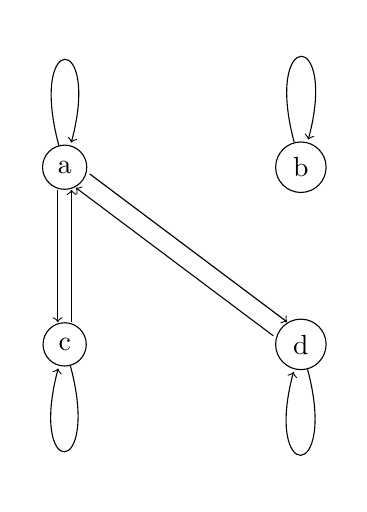
\begin{tikzpicture}[scale=3]
						\tikzstyle{vertex}=[circle,draw=black]
						\node[vertex](v1) at (0,0.75) {a};
						\node[vertex](v2) at (1,0.75) {b};
						\node[vertex](v3) at (0,0) {c};
						\node[vertex](v4) at (1,0) {d};
						\draw[ ->,transform canvas={xshift=-2.5pt,yshift=0pt}](v1) -- (v3);
						\draw[ <-,transform canvas={xshift=2.5pt,yshift=0pt}](v1) -- (v3);
						\draw[ ->,transform canvas={xshift=2.5pt,yshift=2.5pt}](v1) -- (v4);
						\draw[ <-,transform canvas={xshift=-2.5pt,yshift=-2.5pt}](v1) -- (v4);
						\path(v1) edge [loop above] node {}(v1);
						\path(v2) edge [loop above] node {}(v2);
						\path(v3) edge [loop below] node {}(v3);
						\path(v4) edge [loop below] node {}(v4);
					\end{tikzpicture}\\
					It is equivalence, relfexive, symmetric and transtive.	
				\subsection{9.5.22: Determidne if the following graphs is an equivalnce relation}
					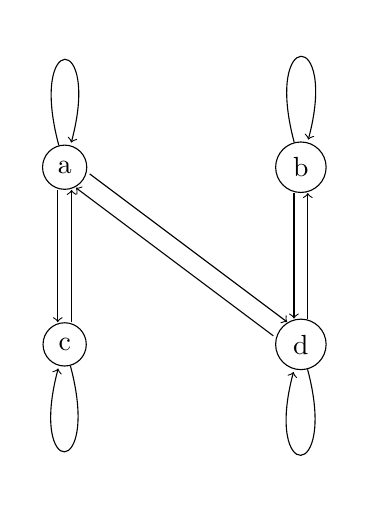
\begin{tikzpicture}[scale=3]
						\tikzstyle{vertex}=[circle,draw=black]
						\node[vertex](v1) at (0,0.75) {a};
						\node[vertex](v2) at (1,0.75) {b};
						\node[vertex](v3) at (0,0) {c};
						\node[vertex](v4) at (1,0) {d};
						\draw[ ->,transform canvas={xshift=-2.5pt,yshift=0pt}](v2) -- (v4);
						\draw[ <-,transform canvas={xshift=2.5pt,yshift=0pt}](v2) -- (v4);
						\draw[ ->,transform canvas={xshift=-2.5pt,yshift=0pt}](v1) -- (v3);
						\draw[ <-,transform canvas={xshift=2.5pt,yshift=0pt}](v1) -- (v3);
						\draw[ ->,transform canvas={xshift=2.5pt,yshift=2.5pt}](v1) -- (v4);
						\draw[ <-,transform canvas={xshift=-2.5pt,yshift=-2.5pt}](v1) -- (v4);
						\path(v1) edge [loop above] node {}(v1);
						\path(v2) edge [loop above] node {}(v2);
						\path(v3) edge [loop below] node {}(v3);
						\path(v4) edge [loop below] node {}(v4);
					\end{tikzpicture}\\
					Is an equivalence class.
				\setcounter{subsection}{40}
				\subsection{9.5.41: Which of these collections of subsets are partitions of $\{1,2,3,4,5,6\}$}
					\subsubsection{$\{1,2\},\{2,3,4\},\{4,5,6\}$}
						Not a partition, since it overlap.	
					\subsubsection{$\{1\},\{2,3,6\},\{4\},\{5\}\}$}
						A partion covers all possinbilities and do not overlap.						
				\setcounter{subsection}{46}
				\subsection{9.5.47: List the ordered pairs in the equivalence relations produced by these partitions of $\{0,1,2,3,4,5\}$}
					\subsubsection{$\{0\},\{1,2\},\{3,4,5\}$}
					  $\{(1,2),(2,1),(3,4),(4,3),(3,5),(5,3),(4,5),(5,4)\}$
				
		\setcounter{chapter}{42}
		\chapter{Uge}
			\section{Afsnit 9.5}
				\subsection{9.5.1: Which of therse relations on $\{0,1,2,3\}$ are equivalence relations? Determine the peoperties of an equivalence relation that the others lack}
					\setcounter{subsubsection}{2}
					\subsubsection{$\{(0, 0), (1, 1), (1, 2), (2, 1), (2, 2), (3, 3)\}$}
						Reflexive, symmetric and transitative
					\subsubsection{$\{(0, 0), (1, 1), (1, 3), (2, 2), (2, 3), (3, 1), (3, 2), (3, 3)\}$}
						Reflexive, symmetric and not transitive
					\subsubsection{$\{(0, 0), (0, 1), (0, 2), (1, 0), (1, 1), (1, 2), (2, 0),(2, 2), (3, 3)\}$}
						Reflexive, not symmetric, transitative
				\setcounter{subsection}{25}
				\subsection{9.5.26: What are the equivalence classes of the equivalence relations in Exercise 1?}
					\setcounter{subsubsection}{2}
					\subsubsection{$\{(0, 0), (1, 1), (1, 2), (2, 1), (2, 2), (3, 3)\}$}
						$\{0\},\{1,2\},\{3\}$
					\subsubsection{$\{(0, 0), (1, 1), (1, 3), (2, 2), (2, 3), (3, 1), (3, 2), (3, 3)\}$}
						$\{0\},\{1,2,3\}$
					\subsubsection{$\{(0, 0), (0, 1), (0, 2), (1, 0), (1, 1), (1, 2), (2, 0),(2, 2), (3, 3)\}$}
						$\{3\},\{0,1,2\}$
				\setcounter{subsection}{1}
				\subsection{9.5.2: Which of these relations on the set of all people are equivalence relations? Determine the properties of an equivalence relation that the others lack.}
					\setcounter{subsubsection}{3}
					\subsubsection{$\{(a,b)|a$ and $b$ have met\}}
						Reflexive, symmetric and not transitive
				\subsection{9.5.3: Which of these relations on the set of all function form $\mathbb{Z}$ to $\mathbb{Z}$ are equivalence relations? Determine tha properties of an equivalence relation that the others lack.}
					\setcounter{subsubsection}{1}
					\subsubsection{$\{(f,g)|f(0)=g(0)$ or $f(1)=g(1)$\}}
						not reflexive, not symmetric, not transitive
					\subsubsection{$\{(f,g)|f(x)-g(x)=1$ for all $x\in \mathbb{Z}\}$}
						not reflexive, not symmetric, not transitive
				\setcounter{subsection}{40}
				\subsection{9.5.41: Which of these collections of subsets are partitions of $\{1,2,3,4,5,6\}$?}
					\setcounter{subsubsection}{2}
					\subsubsection{$\{2,4,6\}.\{1,3,5\}$}
						partition, all elements are in the subsets and no overlap
					\subsubsection{$\{1,4,5\},\{2,6\}$}
						not partition
				\setcounter{subsection}{1}
			\section{Løs følgende tidligere eksamensopgave: Lad $R=\{(a,a),(a,b),(b,c),(d,c)\}$ være en relation på mængden $\{a,b,c,d\}$}
				\subsection{Tegn de orienterede grafer for $R,\color{red} R^2, \color{green}R^3, \color{blue}R^4$ og den transitive lukning $t(R)$}
					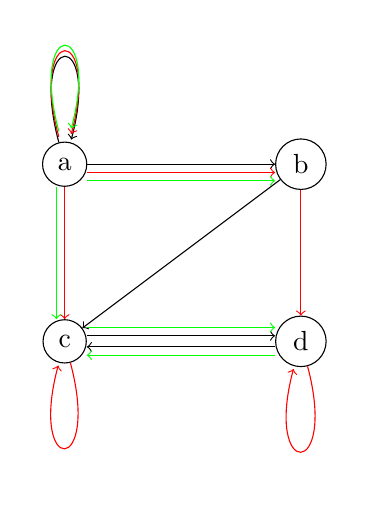
\begin{tikzpicture}[scale=3]
						\tikzstyle{vertex}=[circle,draw=black]
						\node[vertex](v1) at (0,0.75) {a};
						\node[vertex](v2) at (1,0.75) {b};
						\node[vertex](v3) at (0,0) {c};
						\node[vertex](v4) at (1,0) {d};
						\draw[ ->,transform canvas={xshift=0pt,yshift=0pt}](v1) -- (v2);
						\draw[ ->,transform canvas={xshift=0pt,yshift=0pt}](v2) -- (v3);
						\draw[ ->,transform canvas={xshift=0pt,yshift=-2pt}](v4) -- (v3);
						\draw[ ->,transform canvas={xshift=0pt,yshift=2pt}](v3) -- (v4);
						\path(v1) edge [loop above] node {}(v1);
						\path(v1) edge [color=red, loop above,transform canvas={xshift=0pt,yshift=2pt}] node {}(v1);
						\draw[ ->,color=red, transform canvas={xshift=0pt,yshift=-3pt}](v1) -- (v2);
						\draw[ ->,color=red, transform canvas={xshift=0pt,yshift=0pt}](v1) -- (v3);
						\draw[ ->,color=red, transform canvas={xshift=0pt,yshift=0pt}](v2) -- (v4);
						\path(v3) edge [color=red, loop below,transform canvas={xshift=0pt,yshift=0pt}] node {}(v3);
						\path(v4) edge [color=red, loop below,transform canvas={xshift=0pt,yshift=0pt}] node {}(v4);
						\path(v1) edge [color=green, loop above,transform canvas={xshift=0pt,yshift=4pt}] node {}(v1);
						\draw[ ->,color=green, transform canvas={xshift=0pt,yshift=-6pt}](v1) -- (v2);
						\draw[ ->,color=green,transform canvas={xshift=0pt,yshift=-5pt}](v4) -- (v3);
						\draw[ ->,color=green,transform canvas={xshift=0pt,yshift=5pt}](v3) -- (v4);;
						\draw[ ->,color=green, transform canvas={xshift=-3pt,yshift=0pt}](v1) -- (v3);
					\end{tikzpicture}\\
					I $\color{blue}R^4$ bliver der ikke tilføjet nogle nye elementer dermed vil den transitive lukning blive:\\
					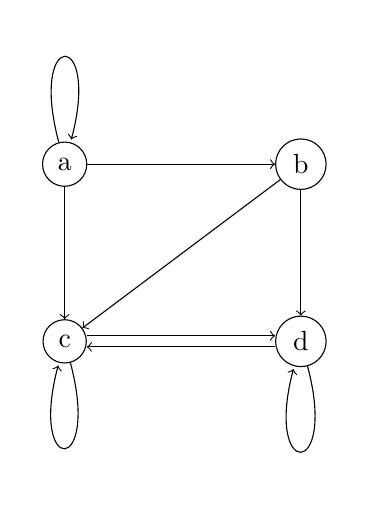
\begin{tikzpicture}[scale=3]
						\tikzstyle{vertex}=[circle,draw=black]
						\node[vertex](v1) at (0,0.75) {a};
						\node[vertex](v2) at (1,0.75) {b};
						\node[vertex](v3) at (0,0) {c};
						\node[vertex](v4) at (1,0) {d};
						\draw[ ->,transform canvas={xshift=0pt,yshift=0pt}](v1) -- (v2);
						\draw[ ->,transform canvas={xshift=0pt,yshift=0pt}](v2) -- (v3);
						\draw[ ->,transform canvas={xshift=0pt,yshift=-2pt}](v4) -- (v3);
						\draw[ ->,transform canvas={xshift=0pt,yshift=2pt}](v3) -- (v4);
						\path(v1) edge [loop above] node {}(v1);
						\draw[ ->, transform canvas={xshift=0pt,yshift=0pt}](v1) -- (v3);
						\draw[ ->, transform canvas={xshift=0pt,yshift=0pt}](v2) -- (v4);
						\path(v3) edge [ loop below,transform canvas={xshift=0pt,yshift=0pt}] node {}(v3);
						\path(v4) edge [loop below,transform canvas={xshift=0pt,yshift=0pt}] node {}(v4);
					\end{tikzpicture}\\
				\subsection{Er t(R)en ækvivalen relation?}
					Not relfexive, not symmetric, transtitative.
			\section{Afsnit 9.6}
				\setcounter{subsection}{0}
				\subsection{9.6.1: Which of these relations on $\{0,1,2,3\}$ are partial orderings? Determine the properties of a partia ordering that the others lack.}
					\subsubsection{$\{(0, 0), (1, 1), (2, 2), (3, 3)\}$}
						reflexive, transitive, antisymmetric
					\subsubsection{$\{(0, 0), (1, 1), (2, 0), (2, 2), (2, 3), (3, 2), (3, 3)\}$}
						Reflexive, transitative, not antisymmetric
				\setcounter{subsection}{4}
				\subsection{9.6.5: Which of these are posets?}
					\subsubsection{$(\mathbb{Z},=)$}
						Reflexive, antisymmetric, transitative
					\subsubsection{$(\mathbb{Z},\neq)$}
						Not relfexive, nto anitsymmetric, not transitative
				\setcounter{subsection}{6}
				\subsection{9.6.7: Determine whether the relations represented by these zero-one matrices are partial orders.}
					\subsubsection{$\begin{bmatrix}
								1 & 1 & 1\\
								1 & 1 & 0\\
								0 & 0 & 1
								\end{bmatrix}$}
						Reflexive, not antisymmetric, not transitative
				\setcounter{subsection}{13}
				\subsection{9.6.14: Which of these pairs of elements are comparable in the poset $(\mathbb{Z}^+,|)$?}
					\subsubsection{5,15}
						True
					\subsubsection{6,9}
						False
				\setcounter{subsection}{17}
				\subsection{9.6.18: Find the lexicographic ordering of these $n$-tuples:}
					\subsubsection{(1,1,2),(1,2,1)}
						(1,1,2),(1,2,1)
					\subsubsection{(0,1,2,3),(0,1,3,2)}
						(0,1,2,3),(0,1,3,2)
					\subsubsection{(1,0,1,0,1),(0,1,1,1,0)}
						(0,1,1,1,0),(1,0,1,0,1)
				\setcounter{subsection}{25}
				\subsection{9.6.26: List all ordered pairs in the partial ordering.}
					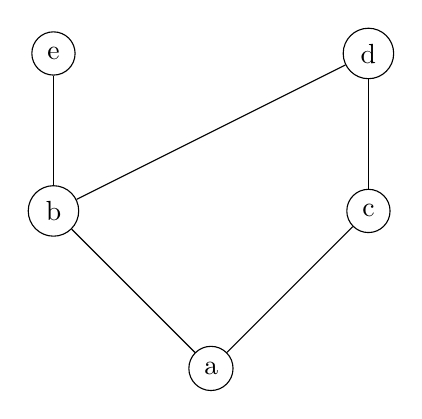
\begin{tikzpicture}[scale=2]
						\tikzstyle{vertex}=[circle,draw=black]
						\node[vertex](v1) at (1,0) {a};
						\node[vertex](v2) at (0,1) {b};
						\node[vertex](v3) at (2,1) {c};
						\node[vertex](v4) at (2,2) {d};
						\node[vertex](v5) at (0,2) {e};
						\draw[-](v1) -- (v2);
						\draw[-](v1) -- (v3);
						\draw[-](v3) -- (v4);
						\draw[-](v2) -- (v4);
						\draw[-](v2) -- (v5);
					\end{tikzpicture}\\
					$(a,b),(a,e),(b,e),(b,d),(a,c),(a,d),(c,d)$
			\setcounter{section}{1}
			\section{Afsnit 9.6}
				\subsection{9.6.1: Which of these relations on $\{0,1,2,3\}$ are partial orderings? Determine the properties of a partia ordering that the others lack.}
					\setcounter{subsubsection}{2}
					\subsubsection{$\{(0,0),(1,1),(1,2),(2,2),(3,3)\}$}
						Reflexive, transitive, antisymmetric
					\subsubsection{$\{(0,0),(1,1),(1,2),(1,3),(2,2),(2,3),(3,3)\}$}
						Reflexive, transitive, antisymmetric
				\setcounter{subsection}{4}
				\subsection{9.6.5: Which of these are posets?}
					\setcounter{subsubsection}{2}
					\subsubsection{$(\mathbb{Z}, \geq )$}
						Reflexive, not transitive, antisymmetric
					\subsubsection{$(\mathbb{Z}, \nmid )$}
						Not reflexive, not transtive, not antisymmetric
				\setcounter{subsection}{13}
				\subsection{9.6.14: Which of these pairs of elements are comparable in the posets ($\mathbb{Z}^+,|$)?}
					\setcounter{subsubsection}{2}
					\subsubsection{$8,16$}
						comparable
					\subsubsection{$7,7$}
						comparable
				\setcounter{subsection}{23}
				\subsection{9.6.24: Draw the Hasse diagram for inclusion on the set $P(S)$, where $S=\{a,b,c\}$}
					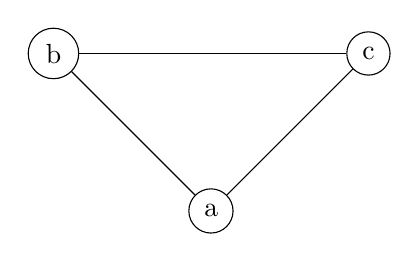
\begin{tikzpicture}[scale=2]
						\tikzstyle{vertex}=[circle,draw=black]
						\node[vertex](v1) at (1,0) {a};
						\node[vertex](v2) at (0,1) {b};
						\node[vertex](v3) at (2,1) {c};
						\draw[-](v1) -- (v2);
						\draw[-](v1) -- (v3);
						\draw[-](v3) -- (v2);
					\end{tikzpicture}
				\setcounter{subsection}{31}
				\subsection{9.6.32: Answer these questions for the partial order represented by this Hasse diagram}
					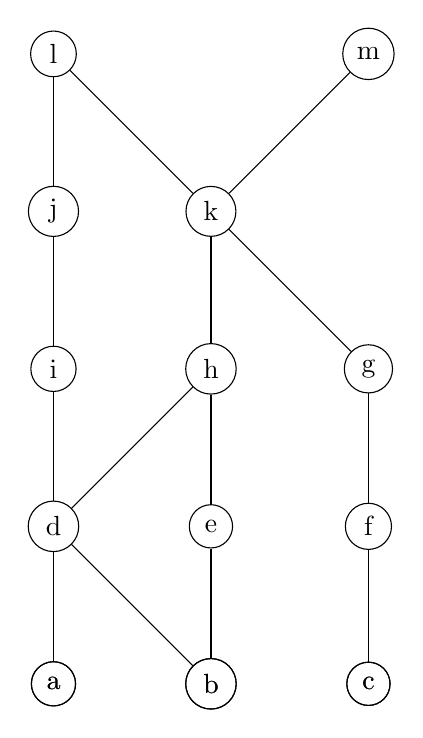
\begin{tikzpicture}[scale=2]
						\tikzstyle{vertex}=[circle,draw=black]
						\node[vertex](v1) at (0,0) {a};
						\node[vertex](v2) at (1,0) {b};
						\node[vertex](v3) at (2,0) {c};
						\node[vertex](v1) at (0,0) {a};
						\node[vertex](v2) at (1,0) {b};
						\node[vertex](v3) at (2,0) {c};
						\node[vertex](v4) at (0,1) {d};
						\node[vertex](v5) at (1,1) {e};
						\node[vertex](v6) at (2,1) {f};
						\node[vertex](v7) at (0,2) {i};
						\node[vertex](v8) at (1,2) {h};
						\node[vertex](v9) at (2,2) {g};
						\node[vertex](v10) at (0,3) {j};
						\node[vertex](v11) at (1,3) {k};
						\node[vertex](v12) at (0,4) {l};
						\node[vertex](v13) at (2,4) {m};
						\draw[-](v1) -- (v4);
						\draw[-](v2) -- (v4);
						\draw[-](v2) -- (v5);
						\draw[-](v3) -- (v6);
						\draw[-](v4) -- (v7);
						\draw[-](v4) -- (v8);
						\draw[-](v5) -- (v8);
						\draw[-](v6) -- (v9);
						\draw[-](v7) -- (v10);
						\draw[-](v8) -- (v11);
						\draw[-](v9) -- (v11);
						\draw[-](v10) -- (v12);
						\draw[-](v11) -- (v12);
						\draw[-](v11) -- (v13);
					\end{tikzpicture}
					\subsubsection{Find the maximal elements}
						$l$ and $m$
					\subsubsection{Find the minimal elements}
						$a,b$ and $c$
					\subsubsection{Is there a greatest element}
						No
					\subsubsection{Is there a least elements}
						No
		\chapter{Uge}
			\section{Afsnit 5.3}
				\setcounter{subsection}{24}
				\subsection{5.3.25: Give a recursive definition of}
					\subsubsection{the set of even integers}
						$S_0 = \{0\}$\\
						$S_n=S_{n-1}\cup\{x+2,x-2|x\in S_{n-1}\},n\geq 1$
					\subsubsection{the set of positive integers congruent to 2 modulo 3}
						$S_0 = \{2\}$\\
						$S_n=S_{n-1}\cup\{x+3|x\in S_{n-1}\},n\geq 1$
					\subsubsection{the set of positive integers not divisible by 5.}
						$S_0 = \{1,2,3,4\}$\\
						$S_n=S_{n-1}\cup\{x+5|x\in S_{n-1}\},n\geq 1$
				\setcounter{subsection}{45}
				\subsection{5.3.46: Use structural induction to show that $l(T)$, the number of leaves of a full binary tree $T$ , is 1 more than $i(T )$, the number of internal vertices of T }
				Basis: $P(S_0$) $S_0=\{$\begin{tikzpicture}
						\node(v1) at (0,0) {.};
				\end{tikzpicture}\}, her er $l(P)=0$ og $i(T)=1$\\
						Ved tilføjelsen af et trin vil et blad blive til en indre knude og der vil komme to nye blade dermed stiger begge med 1 og udligner sig selv.
			\section{Afsnit 4.1}
				\setcounter{subsection}{0}
				\subsection{4.1.1: Does 17 divide each of these numbers?}
					\subsubsection{17|68}
						 yes by 4
					\subsubsection{17|84}
						no
					\subsubsection{17|357}
						yes by 21
					\subsubsection{17|1001}
						no
				\subsection{4.1.2: Prove that if $a$ is an integer other than 0, then}
					$a|b=\exists k in \mathbb{Z}: a\cdot k = b$
					\subsubsection{1 divides $a$}
						$k=a$
					\subsubsection{$a$ divides 0}
						$k=0$
				\subsection{4.1.3 Prove if $a | b$ then $a | bc $ for all integers $c$}
					\begin{align*}
						a|b\rightarrow a|bc, c\in \mathbb{Z}\\
						b=ak\rightarrow a|akc\\
						ak_1c=ak_2\\
						k_2=k_1c
					\end{align*}
			\section{Afsnit 5.3}
				\setcounter{subsection}{25}
				\subsection{5.3.26: Let $S$ be the set of positive integers defined by}
					Basis step: $1\in S$\\
					Recursive step: If $n\in S$, then $3n+2\in S$ and $n^2\in S$.\\
					\subsubsection{Show that if $n\in S$, then $n\equiv 1(mod\; 4)$}
						Basis: $S_0=1 \land 1 (mod\; 4)=1$\\ 
						From here there is two outcomes\\
						$n^2 \in S$ this will result in if $k (mod\; 4$ then $k^2 (mod\;4$\\
						$3n+2\in S$ since the left side is essentialy $(4k+1)$ then $3(4k+1)+2=12k+5$ this shows it will create a multiple of 12 plus 5 and therefore result in 1 when mod.
					\subsubsection{Show that there exists an integer $m\equiv 1 (mod\; 4)$ that does not belong to $S$}
						$m=13$ which will not be in $S$ since recursive step always creates $n_0<n_1$ and the only numbers under 13 is 1 and 5 which will not create 13 in the recursive step.
				\setcounter{subsection}{44}
				\subsection{Ue structural induction to show that $n(T)\geq 2h(T)+1$, where $T$ is a full binary tree $n(T)$ equals the number of vertices of $T$, and $h(T)$ is the height of $T$}
					basis: $n(T_0)=1 \geq 2h(T_)+1 = 1$\\
					For every step the height will get one larger resulting in the right side getting $2$ larger. The rightside will for every step grow in the minimum tree grow $2$ larger, which is equal and in any case where a branch is created which does not add to the height it will simply only grow in vertices.
			\section{4.1}
				\setcounter{subsection}{3}
				\subsection{4.1.4: Prove that part ($iii$) of Theorem 1 is true.}
					Let $a$ and $b$ be integers and let $m$ be a prositve integer. then $a\equiv b (mod\;m)$ if and only if $a\; mod\; m=b\;mod\;m$\\
					\begin{align*}
						a\equiv b \; mod\;m\\
						m|(a-b)=0\\
						a\;mod\;m=b\;mod\;m
					\end{align*}
				\setcounter{subsection}{5}
				\subsection{4.1.6: Show that if $a$,$b$ and $c$ are integers, where $a\neq 0$ and $c\neq 0$ such that $ac |bc$ then $a|b$}
					Since $ac|bc$ if this is true it must be true that $a|b$ due to the first beig the first simply just "strethedi"
				\setcounter{subsection}{7}
				\subsection{4.1.8: Prove or disprove that if $a|bc$ where $a,b$ and $c$ are positive integers and $a\neq 0$ then $a|b$ or $a|c$}
					Disproof by example $9|3\cdot3$ but $9|3$ is not true
				\setcounter{subsection}{12}
				\subsection{What are the quotient and remainder when}
					$a=bq+r$
					\subsubsection{19 is divided by 7}
						$19=7\cdot 2+5$
					\setcounter{subsubsection}{4}
					\subsubsection{0 is divided by 19}
						$0=19\cdot 0 + 0$
					\subsubsection{3 is divided by 5}
						$3=5\cdot 0 + 3$
					\subsubsection{-1 is divided by 3}
						$-1=3\cdot -1+2$
				\setcounter{subsection}{32}
				\subsection{List all integers between -100 and 100 that are congruent to -1 modulo 25}
					$25|(x-(-1)=25|(x+1)$\\
					$x={-1}$\\
					$x_n+25, x_n-25\in x$
			\section{Afsnit 4.3}
				\subsection{4.3.1: Determine whether each of these integers is prime}
					\subsubsection{21}
						$7\cdot 3 = 21$
					\setcounter{subsubsection}{2}
					\subsubsection{111}
						$37\cdot 3 = 111$
				\setcounter{subsection}{2}
				\subsection{4.3.3: Find hte prime factorization of each of these integers}
					\subsubsection{88}
						$2\cdot 2\cdot 2\cdot 11$
					\subsubsection{126}
						$2\cdot 3\cdot 3\cdot 7$
				\setcounter{subsection}{24}
				\subsection{4.3.25: What are the greates common divisors of these pairs of integers?}
					\subsubsection{$3^7\cdot 5^3\cdot 7^3, 2^{11}\cdot 3^5\cdot 5^9$}
					$gcd(3^{min(7,5)}\cdot 5^{min(3,9)})$\\
					$3^5\cdot 5^3=30375$
				\setcounter{subsection}{26}
				\subsection{4.3.27: What are the least common multiple}
					\subsubsection{$3^7\cdot 5^3\cdot 7^3, 2^{11}\cdot 3^5\cdot 5^9$}
					$lcm(3^{max(7,5)}\cdot 5^{max(3,9)}\cdot 2^{11}\cdot7^3)$\\
					$3^9\cdot 5^7\cdot 7^3\cdot 2^{11}=1080203040000000$
			\section{Afsnit 4.1}
				\setcounter{subsection}{20}
				\subsection{4.1.21: Let $m$ be a positive integer. Show that $a\equiv b$ (mod $m$) if $a$ mod $m$=$b$ mod $m$}
					Is this not just the definition of congurence?
				\subsection{4.1.22: Let $m$ be a positive integer. Shot that $a$ mod $m=b$ mod $m$ if $a\equiv b$ (mod $m$)}
		\chapter{Uge}
			\section{Afsnit 4.3}
				\setcounter{subsection}{27}
				\subsection{4.3.28: Find $gcd(1000,625)$ and $lcm(1000,625)$ and verify that $gcd(1000,625)\cdot lcm(1000,625)=1000\cdot 625$.}
					\begin{align*}
						gcd(1000,625)\\
						1000 =  625\cdot 1 + 375\\
						625 = 375 \cdot 1 +250\\
						375=250\cdot 1 +125\\
						250 =125\cdot 2 +0\\
						gcd(1000,625)=125\\[4mm]
						lcm(1000,625)\\
						1000=2\cdot 2\cdot 2\cdot 5\cdot 5\cdot 5=2^3\cdot 5^3\\
						625=5\cdot 5\cdot 5\cdot 5=5^4\\
						lcm(1000,625)=2^3\cdot 5^4=5000\\[4mm]
						lcm(1000,625)\cdot gcd(1000,625)=1000\cdot 625\\
						5000\cdot 125=1000\cdot 625=625000
					\end{align*}
				\setcounter{subsection}{32}
				\subsection{4.3.33: Use the Euclidean algorithm to find}
					\setcounter{subsubsection}{1}
					\subsubsection{$gcd(100,101)$}
						\begin{align*}
							gcd(100,101)\\
							101 = 100\cdot 1 + 1\\
							100 = 1\cdot 100 + 0\\
							gcd(100,101)=1
						\end{align*}
			\section{Afsnit 4.4}
				\subsection{4.4.1: Show that 15 is an inverse of 7 modulo 26}
					$15\cdot 7=105$\\
					$105\% 26=1$
				\setcounter{subsection}{2}
				\subsection{4.4.3: By inspection (as discussed prior to Example 1), find an inverse of 2 modulo 17}
					$2\cdot x \% 27 =1$\\
					$2\cdot 14 \% 27 = 1$
			\setcounter{section}{0}
			\section{Afsnit 4.3}
				\setcounter{subsection}{39}
				\subsection{4.3.40: Express the greates common divisor of easch of these pairs of integers as a linear combination of therse integers}
					\setcounter{subsubsection}{2}
					\subsubsection{35,78}
						\begin{align*}
						gcd(35,78)\\
						78=35\cdot 2 +8\\
						35=8\cdot 4+3\\
						8=3\cdot 2 + 2\\
						3=2\cdot 1 +1\\[4mm]
						1=3-2\cdot 1\\
						2=8-3\cdot 2\\
						3=35-8\cdot 4\\
						8=78-35\cdot 2\\[4mm]
						1=1\cdot 3-1\cdot 2\\
						1=1\cdot 3 - 1\cdot (8-3\cdot 2)\\
						1=1\cdot 3 -(8-3\cdot 2)\\
						1=1\cdot 3 -8+3\cdot 2\\
						1=3\cdot 3 -1\cdot 8\\
						1=-1\cdot 8 + 3\cdot 3\\
						1=-1\cdot 8 + 3\cdot (35-8\cdot 4)\\
						1=-1\cdot 8 + 3\cdot 35 - 8\cdot 12\\
						1=-13\cdot 8 + 3\cdot 35\\
						1=3\cdot 35 - 13\cdot 8\\
						1=3\cdot 35 - 13\cdot (78-35\cdot 2)\\
						1=3\cdot 35 - 78\cdot 13 + 35\cdot 26\\
						1=29\cdot 35 - 78\cdot 13\\
						\end{align*}
			\section{Afsnit 4.4}
				\setcounter{subsection}{4}
				\subsection{4.4.5: Find an inverse of $a$ modulo $m$ for each of these pairs of relatively prime integers using the method followed in Example 2}
					\subsubsection{$a=4,m=9$}
						\begin{align*}
							gcd(4,9)\\
							9=4\cdot 2 + 1\\
							1=9\cdot 1 - 4\cdot 2\\
							\bar{a}=2
						\end{align*}
					\subsubsection{$a=19,m=141$}
							\begin{align*}
								gcd(19,141)\\
								141=19\cdot 7+8\\
								19 = 8\cdot 2 + 1\\
								1=19-2\cdot 8\\
								1=19-2\cdot(141-19\cdot 7)\\
								1=19-141\cdot 2 +19\cdot 14\\
								1=19\cdot 15-141\cdot 2\\
								\bar{a}=15
							\end{align*}
				\setcounter{subsection}{8}
				\subsection{4.4.9: Solve the congruence $4x\equiv 5$ (mod 9) using the inverse of 4 modulo 9 found un part a of Exercise 5}
					$4x\equiv 5$ mod 9\\
					$x\equiv 5\cdot 2$ mod 9\\
					$x\equiv 10$ mod 9
			\section{Afsnit 4.3}
				\setcounter{subsection}{11}
				\subsubsection{4.3.12: Prove that for every positive integer $n$, there are $n$ consecutive composite integers}
				We know that any number can be composed by prime numbers except other prime numbers. But in this statement prime numbers may just be described as itself multiplied by 1.
				\setcounter{subsection}{4}
				\subsection{4.3.5: Find the prime factorization of $10!$.}
					\begin{align*}
						10!&=\\
						   &=1\cdot 2\cdot 3\cdot 4\cdot 5\cdot 6\cdot 7 \cdot 8 \cdot 9\\
						   &=1\cdot 2 \cdot 3 \cdot (2\cdot 2)\cdot 5 \cdot (2\cdot 3) \cdot 7 \cdot (2^3) \cdot (3^2)\\
						   &=2^7\cdot 3^4 \cdot 5 \cdot 7
					\end{align*}
				\subsection{4.3.6: How many zeros are there at the end of $100!$?}
					24 counted by wolfram calculation.	
		\chapter{Uge}
			\section{Afsnit 4.4}
				\setcounter{subsection}{20}
				\subsection{Use the construction in the proof of the Chinese remainder theorem to find all solutions to the system of congruences $x\equiv 1$ (mod 2), $x\equiv 2$ (mod 3), $x\equiv 3$ (mod 5), and $x\equiv 4$ (mod 11).}
					\begin{align*}
						a_1=1\\
						a_2=2\\
						a_3=3\\
						a_4=4\\
						M_1=165\\
						M_2=110\\
						M_3=66\\
						M_4=30\\
						M=330\\[4mm]
						165y_1\equiv 1\;(mod\;2)\\
						y_1\equiv 1\;(mod\;2)\\
						110y_2\equiv 1\;(mod\;3)\\
						2y_2\equiv 1 \;(mod\;3)\\
						y_2\equiv 2\;(mod\;3)\\
						66y_3\equiv 1\;(mod\;5)\\
						y_3\equiv 1\;(mod\;5)\\
						30y_4\equiv 1\;(mod\;11)\\
						8y_4\equiv 1\;(mod\;11)\\
						y_4\equiv 7\;(mod\;11)\\[4mm]
					\end{align*}
					\begin{align*}
						b_1=165\cdot 1 = 65\\
						b_2=110\cdot 2 = 220\\
						b_3=66\cdot 1 = 66\\
						b_4=30\cdot 7 = 210\\[4mm]
						x=165\cdot 1 + 220\cdot 2 + 66\cdot 3 + 210\cdot 4\\
						x=165+440+198+840\\
						x=1643\\
						x\equiv 1643\;(mod\;330)\\
						x\equiv 323\;(mod\;330)
				\end{align*}
			\setcounter{subsection}{30}
			\subsection{4.4.31: Which integers leave a remainder of 1 when divided by 2 and also leave a remainder of 1 when divided 3?}
				$(2\cdot 3)k+1$ where $k\in\mathbb{Z}^+$
			\setcounter{subsection}{32}
			\subsection{4.4.33: Use Fermats little theorem to find $7^{121}$ mod 13}
				$7^{121}=7^{120}\cdot 7$\\
				$7^{121}$ mod 13 $=7$ mod 13
		\section{Afsnit 2.6}
			\subsection{2.6.1: Let $A=\begin{bmatrix}1&1&1&3\\2&0&4&6\\1&1&3&7\end{bmatrix}$.}
				\subsubsection{What size is $A$}
					$3\times 4$
				\subsubsection{What us the third coloumn of $A$}
					$\begin{bmatrix}1\\4\\3\end{bmatrix}$
				\subsubsection{What is the second row of $A$}
					$\begin{bmatrix}2&0&4&6\end{bmatrix}$
				\subsubsection{What is the element of $A$ in the (3,2)th position}
					$1$
				\subsubsection{What is $A^t$}
					$\begin{bmatrix}1&2&1\\1&0&1\\1&4&3\\3&6&7\end{bmatrix}$
			\subsection{2.6.2: Find $A+B$ where}
				\subsubsection{$A=\begin{bmatrix}1&0&4\\-1&2&2\\0&-2&-3\end{bmatrix},B=\begin{bmatrix}-1&3&5\\2&2&-3\\2&-3&0\end{bmatrix}$.}
					$\begin{bmatrix}0&3&9\\1&4&-1\\2&-5&-3\end{bmatrix}$
				\subsubsection{$A=\begin{bmatrix}-1&0&5&6\\-4&-3&5&-2\end{bmatrix}, B=\begin{bmatrix}-3&9&-3&4\\0&-2&-1&2\end{bmatrix}$}
					$\begin{bmatrix}-4&9&2&10\\-4&-5&4&0\end{bmatrix}$
			\subsection{2.6.3: Find AB if}
				\subsubsection{$A=\begin{bmatrix}2&1\\3&2\end{bmatrix}, B=\begin{bmatrix}0&4\\1&3\end{bmatrix}$}
					$AB=\begin{bmatrix}1&11\\2&18\end{bmatrix}$
			\setcounter{subsection}{4}
			\subsection{2.6.5: Find a mtrix $A$ such that}
				$$\begin{bmatrix}2&3\\1&4\end{bmatrix}A=\begin{bmatrix}3&0\\1&2\end{bmatrix}$$
				\begin{align*}
					2\cdot x +3\cdot y =3\\
					1\cdot x +4\cdot y =1\\
					x=\frac{9}{5}\\
					y=-\frac{1}{5}\\
					2x+3y=0\\
					x+4y=2\\
					y=\frac{4}{5}\\
					x=-\frac{6}{5}
				\end{align*}
				$\begin{bmatrix}\frac{9}{5}&-\frac{6}{5}\\-\frac{1}{5}&\frac{4}{5}\end{bmatrix}$
			\setcounter{subsection}{17}
			\subsection{2.6.18: Show that}
				$$\begin{bmatrix}2&3&-1\\1&2&1\\-1&-1&3\end{bmatrix}$$
				Is the inverse of
				$$\begin{bmatrix}7&-8&5\\-4&5&-3\\1&-1&1\end{bmatrix}$$
				$$\begin{bmatrix}14-8-5&21-16-5&-7-8+15\\-8+5+3&-12+10+3&4+5-9\\2-1-1&3-2-1&-1-1+3\end{bmatrix}$$
				$$\begin{bmatrix}1&0&0\\0&1&0\\0&0&1\end{bmatrix}$$
		\setcounter{section}{1}
		\section{Afsnit 4.4}
			\setcounter{subsection}{25}
			\subsection{Find all solutions, if any to the system of congruences $x\equiv 5$ (mod 6), $x\equiv 4$ (mod 12) and $x\equiv 8$ (mod 15)}
				\begin{align*}
					a_1=5\\
					a_2=4\\
					a_3=8\\
					m_1=180\\
					m_2=90\\
					m_3=72\\
					m=1080\\[4mm]
					180y_1\equiv 1\;(mod\;6)\\
					0\equiv 1\;(mod\;6)\\
					90y_2\equiv 1\;(mod\;12)\\
					6y_2\equiv 1\;(mod\;12)\\
					y_2\equiv 6\;(mod\;12)\\
					72y_3\equiv 1\;(mod\;15)\\
					y_3\equiv 7\;(mod\;15)\\[4mm]
					b_1=180\cdot 0=0\\
					b_2=90\cdot 2 = 180\\
					b_3=72\cdot 7 = 504\\[4mm]
					x=0+180\cdot 4 + 504\cdot 8\\
					x=4752\\
					x\equiv4752\;(mod\;1080)\\
					x\equiv 432\;(mod\;1080)
				\end{align*}
			\setcounter{subsection}{36}
			\subsection{4.4.37}
			\subsubsection{Show that $2^{340}\equiv 1\;(mod\;11)$ by Fermats little theorem and noting that $2^{340}=(2^{10})^{34}$}
				Since 11 is prime and $11\nmid 2$ will $2^{11-1}\equiv 1$ (mod 11).\\
				And $(2^{10})^{34}=2^{340}$ therefore it will be equivalent to 1.
			\subsubsection{Show that $2^{340}\equiv 1\;(mod\;31)$using the fact that $2^{340}=(2^5)^{68}=32^{68}$}
			Since $2^{340}=32^{68}$ therefore it is essentieally $32 \equiv 1$ mod(31) which is true\\ 
			\subsubsection{COnclude from parts (a) and (b) that $2^{340}\equiv 1\;(mod\;341)$.}
				Since 341 is a multiple of 11 it will and we know that $2^{340}$ is $equiv 1$ with 11 it will here also be $\equiv 1$ mod 341.
	\section{Afsnit 2.6}
		\setcounter{subsection}{9}
		\subsection{Let $A$ be a $3\times 4$ matrix, $B$ be a $4\times 5$ matrix, and $C$ be a $4 \times 4$ matrix. Determine which if the following products are defined and find the size of those that are defined}

			\subsubsection{$AB$}
				Not defined
			\subsubsection{$BA$}
				Defined $4\times 4$
			\subsubsection{$AC$}
				Not defined
			\subsubsection{$CA$}
				Defined $4\times 4$
			\subsubsection{$BC$}
				Defined $4\times 4$
			\subsubsection{$CB$}
				Not defined
		\setcounter{subsection}{13}
		\subsection{In this exercise we show that matrix multiplication is associative. Suppose that $A$ is an $m\times p$ matrix, $B$ is a $p\times k$ matrix and $C$ is a $k\times n$ matrix. Show that $A(BC)=(AB)C$}
			For this I will just look at the first index.\\
			Lets say all matric is a two my two for simplicity\\
			For $A(BC)$ the first corner will be $(B_1\cdot C_1)\cdot A_1 + (B_2\cdot C_2)\cdot A_2$\\
			It can here be seen that the parenthesis is not needed and the therefore the multiplication is associative.
		\subsection{Let $$A=\begin{bmatrix}1&1\\0&1\end{bmatrix}$$ Find a formula for $A^n$, whenever $n$ is a positive integer}
			$$A^2=\begin{bmatrix}1&2\\0&1\end{bmatrix}$$
			$$A^3=\begin{bmatrix}1&3\\0&1\end{bmatrix}$$
			$$A^n=\begin{bmatrix}1&n\\0&1\end{bmatrix}$$
	\setcounter{section}{0}
	\section{Afsnit 10.1}
		\setcounter{subsection}{9}
		\subsection{For each undirected graph in Exercises 3-5 that is not simple, find a set of edges to remove to make it simple}
			\setcounter{subsubsection}{2}
			\subsubsection{3}
				$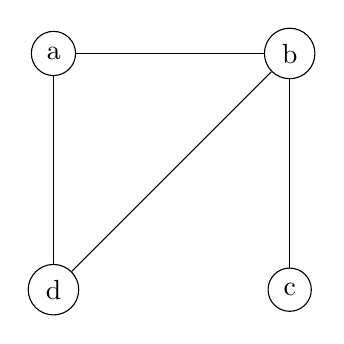
\begin{tikzpicture}[scale=3]
						\tikzstyle{vertex}=[circle,draw=black]
						\node[vertex](v1) at (0,0){d};
						\node[vertex](v2) at (1,0){c};
						\node[vertex](v4) at (0,1) {a};
						\node[vertex](v3) at (1,1) {b};
						\path[-]
							(v2) edge node {}(v3)
							(v4) edge node {}(v1)
							(v3) edge node {}(v4)
							(v3) edge node {}(v1);
					\end{tikzpicture}$\\
					Remove $c,b$
			\subsubsection{4}
			$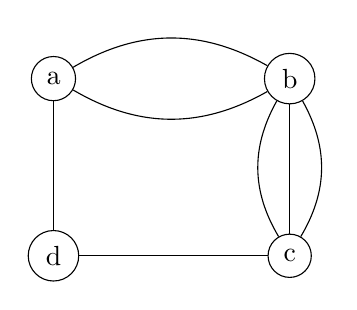
\begin{tikzpicture}[scale=3]
					\tikzstyle{vertex}=[circle,draw=black]
					\node[vertex](v1) at (0,0.75) {a};
					\node[vertex](v2) at (1,0.75) {b};
					\node[vertex](v3) at (1,0) {c};
					\node[vertex](v4) at (0,0) {d};
   					\draw (v1) to [bend right=-30] (v2);
   					\draw (v1) to [bend right=30] (v2);
					\draw (v1) to (v4);
   					\draw (v4) to [text={"e_1"}] (v3);
   					\draw (v2) to [bend left=30, text={"e_3"}] (v3);
   					\draw (v2) to [bend right=30] (v3);
					\draw (v2) -- (v3) node [midway] {};
				\end{tikzpicture}$\\
					Remove 1x $a,b$, 2x$b,c$
			\subsubsection{5}
				$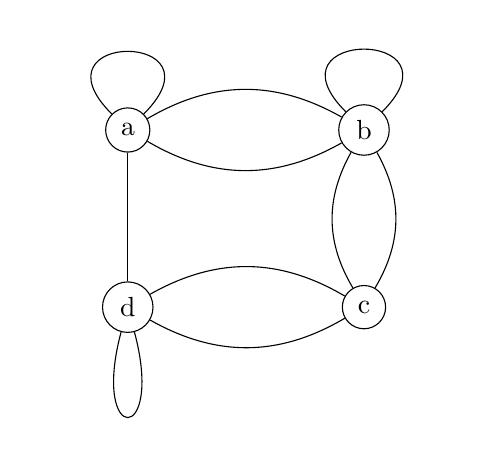
\begin{tikzpicture}[scale=3]
					\tikzstyle{vertex}=[circle,draw=black]
					\node[vertex](v1) at (0,0.75) {a};
					\node[vertex](v2) at (1,0.75) {b};
					\node[vertex](v3) at (1,0) {c};
					\node[vertex](v4) at (0,0) {d};
   					\draw (v1) to [bend right=-30] (v2);
   					\draw (v1) to [bend right=30] (v2);
   					\draw (v4) to [bend right=-30] (v3);
   					\draw (v4) to [bend right=30] (v3);
					\draw (v1) to (v4);
   					\draw (v2) to [bend left=30, text={"e_3"}] (v3);
   					\draw (v2) to [bend right=30] (v3);
					\draw(v1) to [loop] node {}(v1);
					\draw(v2) to [loop] node {}(v2);
					\draw(v4) to [loop below] node {}(v4);
				\end{tikzpicture}$\\
				Remove $a,a$,$b,b$,1x$b,c$,$d,d$,1x $d,c$
	\section{Afsnit 10.2}
		\subsection{Find the number of vertices, edges and degrees of each vertex}
			$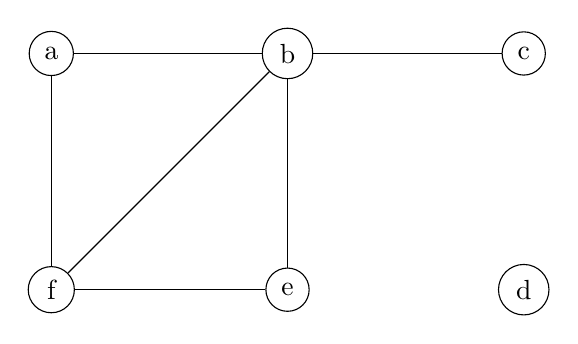
\begin{tikzpicture}[scale=3]
					\tikzstyle{vertex}=[circle,draw=black]
					\node[vertex](v1) at (0,0){f};
					\node[vertex](v2) at (1,0){e};
					\node[vertex](v4) at (0,1) {a};
					\node[vertex](v3) at (1,1) {b};
					\node[vertex](v5) at (2,1) {c};
					\node[vertex](v6) at (2,0) {d};
					\path[-]
						(v2) edge node {}(v3)
						(v4) edge node {}(v1)
						(v3) edge node {}(v4)
						(v3) edge node {}(v1)
						(v1) edge node {} (v2)
						(v3) edge node {} (v5);
				\end{tikzpicture}$\\
				6 vertices\\
				6 edges\\
				a - 2\\
				b - 4\\
				c - 1\\
				e - 2\\
				f - 3
		\setcounter{subsection}{6}
		\subsection{How many edges, vertices and out and in degrees}
			$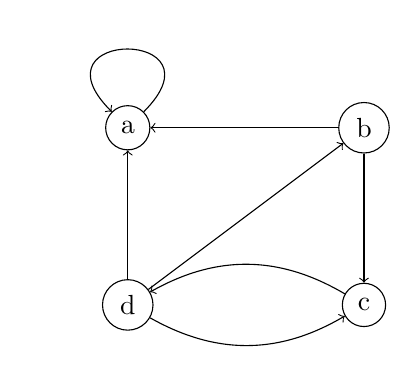
\begin{tikzpicture}[scale=3]
				\tikzstyle{vertex}=[circle,draw=black]
				\node[vertex](v1) at (0,0.75) {a};
				\node[vertex](v2) at (1,0.75) {b};
				\node[vertex](v3) at (1,0) {c};
				\node[vertex](v4) at (0,0) {d};
				\draw[->] (v4) to [bend right=-0] (v2);
				\draw[->](v2) to [bend right=0] (v1);
				\draw[->] (v4) to [bend right=30] (v3);
				\draw[->] (v3) to [bend right=30] (v4);
				\draw[->] (v4) to (v1);
				\draw[->] (v2) to [bend right=0] (v3);
				\draw[->](v1) to [loop] node {}(v1);
			\end{tikzpicture}$\\
			4 vertices\\
			7 edges\\
			a - 3 in 1 out
			b - 1 in 2 out
			c - 2 in 1 out
			d - 1 in 3 out
		\setcounter{subsection}{20}
		\subsection{Determine if the graph is bipartite}
			\begin{figure}[h!]
				\centering
				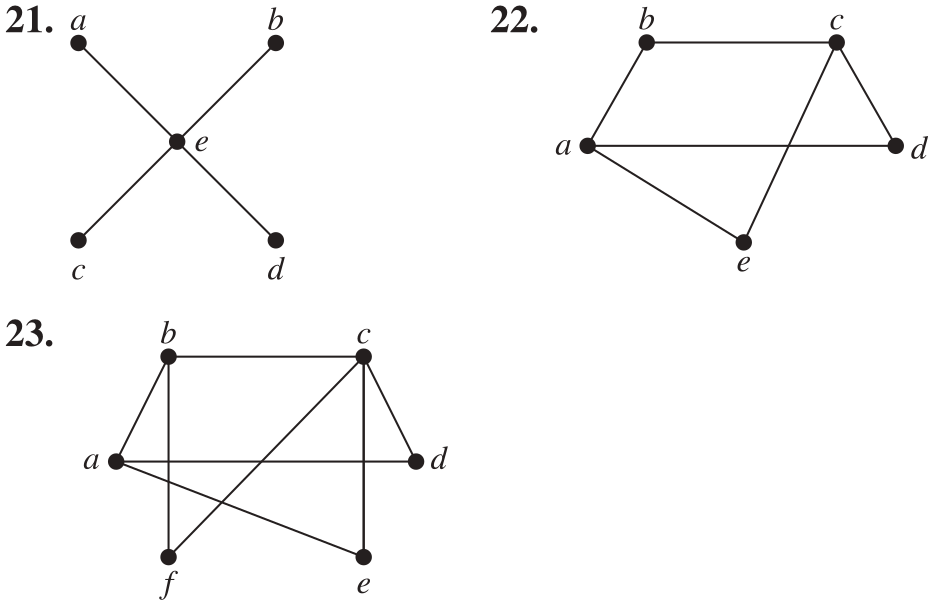
\includegraphics[width=\linewidth]{assets/10,3,21-23.png}
				\label{graphs10.3}
				\caption{Graphs for the following exercises}
			\end{figure}
			\subsubsection{21}
				Bipartite if e is something else than the rest
			\subsubsection{22}
				Bipartite - a c and b d e
			\subsubsection{23}
				Not bipartiple due to b c f
	\section{10.3}
		\subsection{Use adjacency list and matrix to represent the given graph}
			$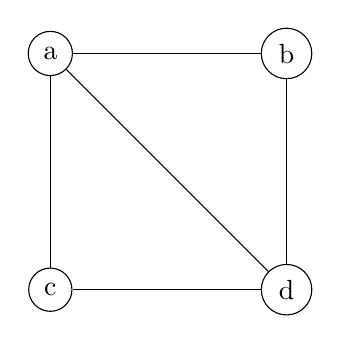
\begin{tikzpicture}[scale=3]
						\tikzstyle{vertex}=[circle,draw=black]
						\node[vertex](v1) at (0,0){c};
						\node[vertex](v2) at (1,0){d};
						\node[vertex](v4) at (0,1) {a};
						\node[vertex](v3) at (1,1) {b};
						\path[-]
							(v2) edge node {}(v3)
							(v4) edge node {}(v1)
							(v3) edge node {}(v4)
							(v4) edge node {}(v2)
							(v1) edge node {} (v2);
					\end{tikzpicture}$\\
			$\begin{bmatrix}
				0&1&1&0\\
				1&0&0&1\\
				1&0&0&1\\
				1&1&1&0
			\end{bmatrix}$
			a - b,d,c\\
			b - a,d\\
			c - a,d\\
			d - a,b,c
		\clearpage
		\setcounter{subsection}{2}
		\subsection{Use adjaceny listi and matrix to represent the given graph}
			\begin{figure}[h!]
				\centering
				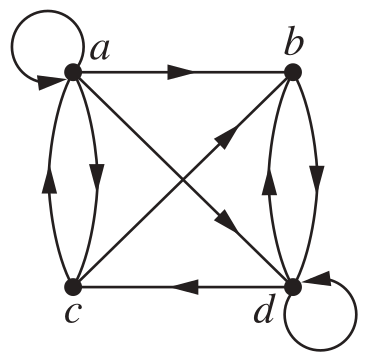
\includegraphics[width=150px]{assets/10,3,3.png}
				\label{10,3,3}
				\caption{Graphs for the following exercise}
			\end{figure}
			$\begin{bmatrix}
				1&1&1&1\\
				0&0&0&1\\
				1&1&0&0\\
				0&1&1&1
			\end{bmatrix}$\\
			a - a,b,c,d\\
			b - d\\
			c - a,b\\
			d - c,b,d
	\setcounter{section}{0}
	\section{Afsnit 10.2}
		\setcounter{subsection}{1}
		\subsection{Number of vertices, edges and degree}
			\begin{figure}[h!]
				\centering
				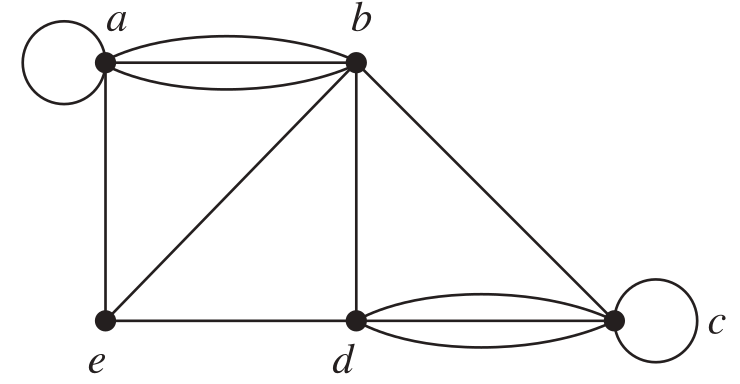
\includegraphics[width=150px]{assets/10,3,2.png}
				\label{10,3,2}
				\caption{Graphs for the following exercise}
			\end{figure}
			5 vertices\\
			13 edges\\
			a - 6\\
			b - 6\\
			c - 6\\
			d - 5\\
			e - 3
		\setcounter{subsection}{4}
		\subsection{Can a simple graph exist with 15 vertices each of degree 5}
			yes since for 3 vertices 3 edges exist 4 has max 6 and 5 has max 9\\
			Therefor the max edges for 15 is 42 and therefore all vertices can have a total of 82 degrees. Which is 5 to each and two can actually have 6\\
		\setcounter{subsection}{10}
		\subsection{How does one make a underlying graph}
			Take a graph and remove all directions
		\setcounter{subsection}{25}\clearpage
		\subsection{Determine biparity}
			\begin{figure}[h!]
				\centering
				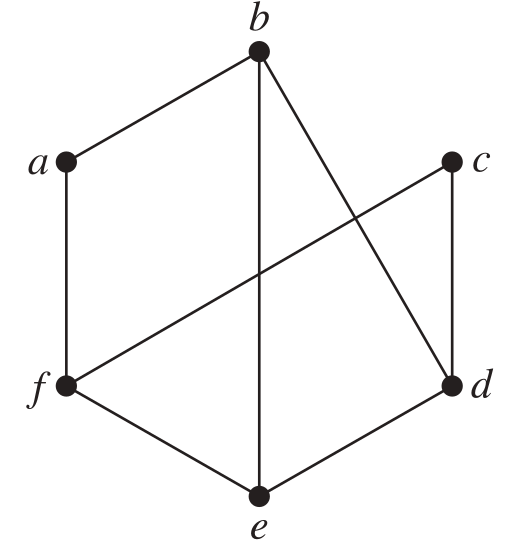
\includegraphics[width=150px]{assets/10,2,25.png}
				\label{10,2,25}
				\caption{Graphs for the following exercise}
			\end{figure}
			Not parible due to b e d
	\section{Afsnit 10.3}
		\setcounter{subsection}{37}
		\subsection{Is the given pair isomorphic}
			\begin{figure}[h!]
				\centering
			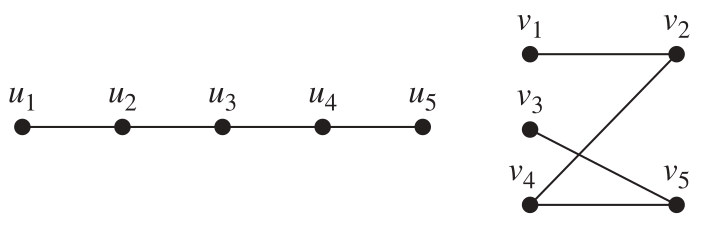
\includegraphics[width=200px]{assets/10,3,38.png}
				\label{}
				\caption{Graphs for the following exercises}
			\end{figure}
			Yes $u_n\rightarrow v_n$\clearpage
		\setcounter{subsection}{39}
		\subsection{Is the given pair isomorphic}
			\begin{figure}[h!]
				\centering
			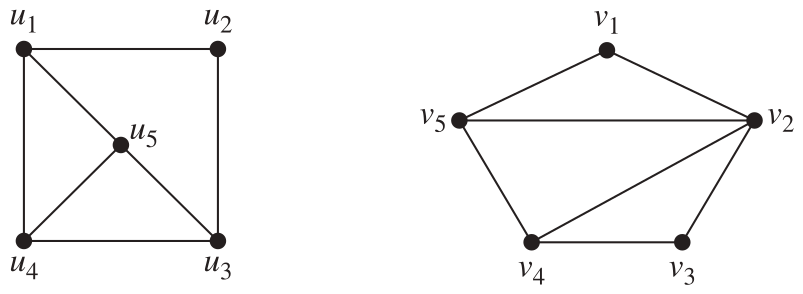
\includegraphics[width=200px]{assets/10,3,40.png}
				\label{}
				\caption{Graphs for the following exercises}
			\end{figure}
			No $v_2$ has 4 degree which non of the graph $U$ has
\chapter{Uge}
	\section{Afsnit 10.2}
		\setcounter{subsection}{17}
		\subsection{Show that in a simple graph with at least two vertices there must be two vertices that have the same degree.}
			Induktion proof\\
			basis: A graph with two vertices with one edge between, both vertices have the same degree.\\
			Step: A vertice can be added. It here can get attached by a minimum to one of the vertices, which results in the two vertices having the same degree. If connected to both it will simply have the same degree as the other.\\
			Therefore it is not possible to add vertices and not have at least two vertices with the same degrees.\\
			A vertice kan have $0\leq d(v)\leq |v|-1$ so a graph with 1 vertice it will have 0 degrees.\\
			Therefore a graph with $d(v_{|v|-1}$ will have $|v|-1$ degrees and the graph with $d(v_{|v|})$ has to have the same amount of degrees as another vertice.
		\subsection{Use Exercise 18 to show that in a group of people, there must be two people who are friends with the same number of other people in the group}
			Assuming that the graph of the group of people is connected. As pr proof from Exercise 18 there will be people with the same amount of friends.
		\setcounter{subsection}{61}
		\subsection{If $G$ is asimple graph with 16 edges and $\bar{G}$ has 13 edges, how many vertices does $G$ have}
			$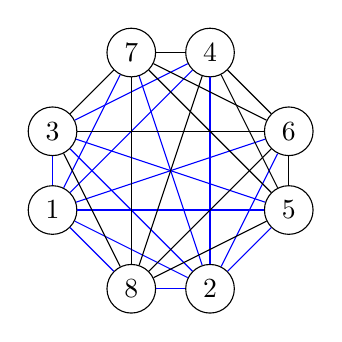
\begin{tikzpicture}[scale=1]
				\tikzstyle{vertex}=[circle,draw=black]
				\node[vertex](v1) at (0,0){1};
				\node[vertex](v2) at (2,-1){2};
				\node[vertex](v3) at (0,1){3};
				\node[vertex](v4) at (2,2){4};
				\node[vertex](v5) at (3,0){5};

				\node[vertex](v6) at (3,1){6};
				\node[vertex](v7) at (1,2){7};
				\node[vertex](v8) at (1,-1){8};
				\path[-]
					(v1) edge[color=blue] node {}(v2)
					(v1) edge[color=blue] node {}(v3)
					(v1) edge[color=blue] node {}(v4)
					(v1) edge[color=blue] node {}(v5)
					(v1) edge[color=blue] node {}(v6)
					(v1) edge[color=blue] node {}(v7)
					(v1) edge[color=blue] node {}(v8)
					(v2) edge[color=blue] node {}(v3)
					(v2) edge[color=blue] node {}(v4)
					(v2) edge[color=blue] node {}(v5)
					(v2) edge[color=blue] node {}(v6)
					(v2) edge[color=blue] node {}(v7)
					(v2) edge[color=blue] node {}(v8)
					(v3) edge[color=blue] node {}(v4)
					(v3) edge[color=blue] node {}(v5)
					(v3) edge node {}(v6)
					(v3) edge node {}(v7)
					(v3) edge node {}(v8)
					(v4) edge node {}(v5)
					(v4) edge node {}(v6)
					(v4) edge node {}(v7)
					(v4) edge node {}(v8)
					(v5) edge node {}(v6)
					(v5) edge node {}(v7)
					(v5) edge node {}(v8)
					(v6) edge node {}(v7)
					(v6) edge node {}(v8)
					(v7) edge node {}(v8);
			\end{tikzpicture}$\\
			$K_n$=28 kanter\\
			$K_n=\frac{n(n-1)}{2}$\\
			$K_8=28$
	\section{Afsnit 10.3}
		\setcounter{subsection}{38}
		\subsection{Is the given graph isomorphic}
			\begin{figure}[h!]
				\centering
				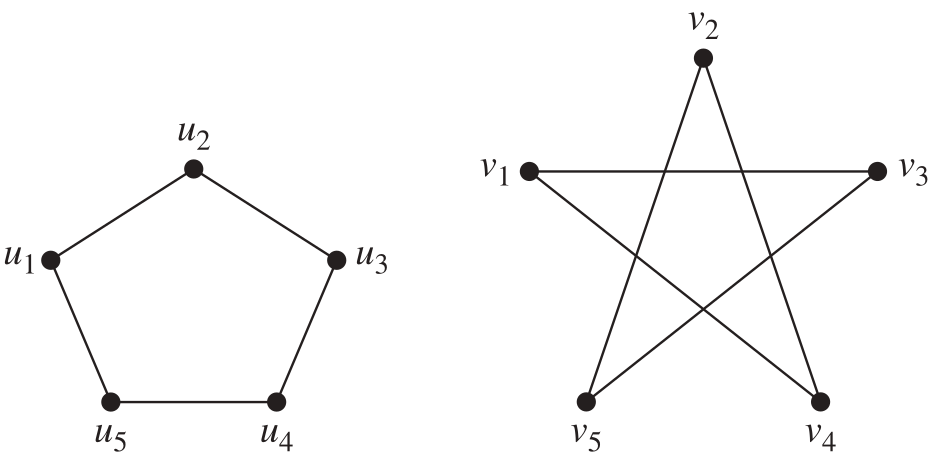
\includegraphics[width=200px]{assets/10,3,39.png}
				\label{}
				\caption{}
			\end{figure}
			$u_1\rightarrow v_1,u_5\rightarrow v_4,u_4\rightarrow v_2,u_3\rightarrow v_5, u_2\rightarrow v_3$
		\setcounter{subsection}{41}
		\subsection{Is the given graph isomorphic}
			\begin{figure}[h!]
				\centering
				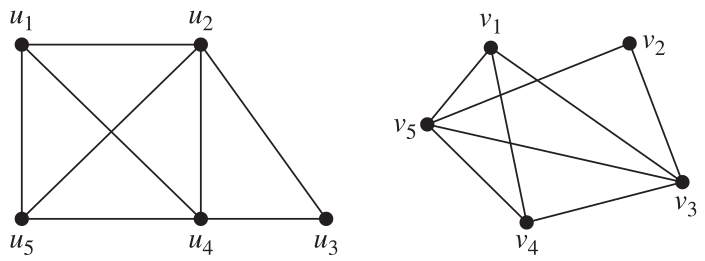
\includegraphics[width=200px]{assets/10,3,42.png}
				\label{}
				\caption{}
			\end{figure}
		 	$u_2\rightarrow v_3$\\
			$u_4\rightarrow v_5$\\
			$u_3\rightarrow v_2$\\
			$u_1\rightarrow v_1$\\
			$u_5\rightarrow v_4$
		\setcounter{subsection}{48}
		\subsection{Show that isomorphism if simple graphs is an equivalence relation}
			A graph is reflexive (its isomorph with itself)\\
			Symetric if a mapping exist one way the inverse exists\\
			Transitive. If a mapping exist to a graph and a mapping exist then the combined mapping exists.
	\section{Afsnit 10.4}
		\setcounter{subsection}{2}
		\subsection{Determinde if the graph is connected}
			\begin{figure}[h!]
				\centering
			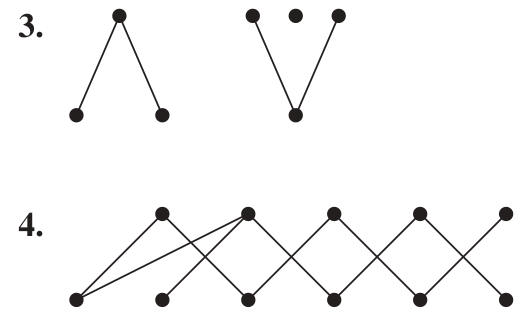
\includegraphics[width=200px]{assets/10,4,3-4.png}
				\label{}
				\caption{}
			\end{figure}
			No it got 3 connected components
		\subsection{Determinde if the graph is connected}
			Yes
	\setcounter{section}{1}
	\section{Afsnit 10.4}
		\subsection{Does each of these lists of vertices form a path in the following graph? Which paths are simple? Which are circuits? What are the lengths of those that are paths?}
			\begin{figure}[h!]
				\centering
				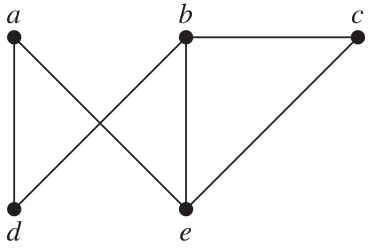
\includegraphics[width=150px]{assets/10,4,1.png}
				\label{}
				\caption{}
			\end{figure}	
			\subsubsection{$a,e,b,c,b$}
				Not simple path with the length of 3
			\subsubsection{$a,e,a,d,b,c,a$}
				Not a path no edge from c to a
			\subsubsection{$e,b,a,d,b,e$}
				Not a path no edge from b to a
			\subsubsection{$c,b,d,a,e,c$}
				Simple path with the length of 5
		\setcounter{subsection}{4}
		\subsection{Are the following graph connected}
			\begin{figure}[h!]
				\centering
				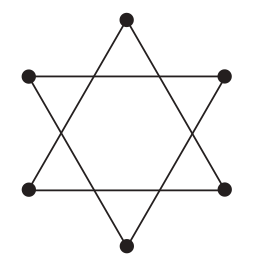
\includegraphics[width=150px]{assets/10.4.5.png}
				\label{}
				\caption{}
			\end{figure}
			Not connected	
		\subsection{How many connected component does 10.4.3-5 have}
			10.4.3 - 3\\
			10.4.4 - 1\\
			10.4.5 - 2
		\setcounter{subsection}{11}
		\subsection{Determine whter each of these graphs is stringly connected and if not wheter it is weakly connected}
			\subsubsection{}
				\begin{figure}[h!]
					\centering
					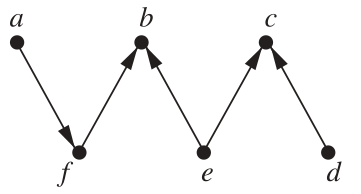
\includegraphics[width=150px]{assets/10,4,12,a.png}
					\label{}
				\caption{Graphs for the following exercise}
				\end{figure}
				It is weakly connected, due to b and c not connecting	
		\setcounter{subsection}{13}
		\subsection{Find the stringly connected components of each of these graphs}
			\subsubsection{}
				\begin{figure}[h!]
					\centering
					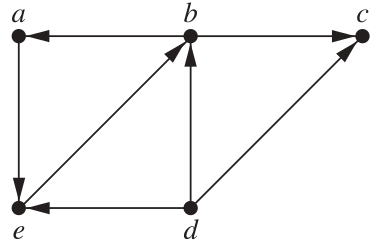
\includegraphics[width=150px]{assets/10,4,14,a.png}
					\label{}
				\caption{Graphs for the following exercise}
				\end{figure}
				$b,a,e,c$\\
				$d,b,e,c,a$
	\section{Afsnit 11.1}
		\subsection{Which of theese is trees}
			\begin{figure}[h!]
				\centering
				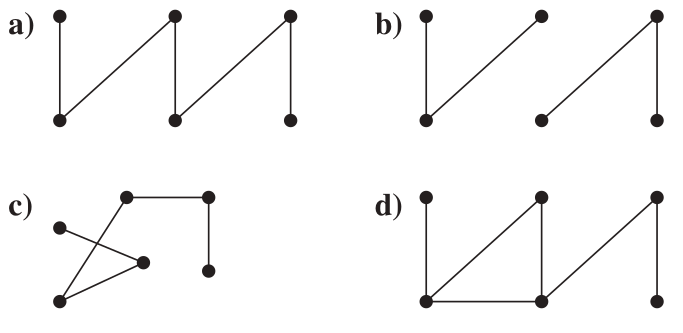
\includegraphics[width=200px]{assets/11,1,1.png}
				\label{}
				\caption{Graphs for the following exercise}
			\end{figure}	
			\subsubsection{}
				Tree
			\subsubsection{}
				Not tree not connected
			\setcounter{subsubsection}{3}
			\subsubsection{}
				Not tree loop
		\setcounter{subsection}{2}
		\subsection{Answer these questions about the rooted tree illustrated}
			\begin{figure}[h!]
				\centering
				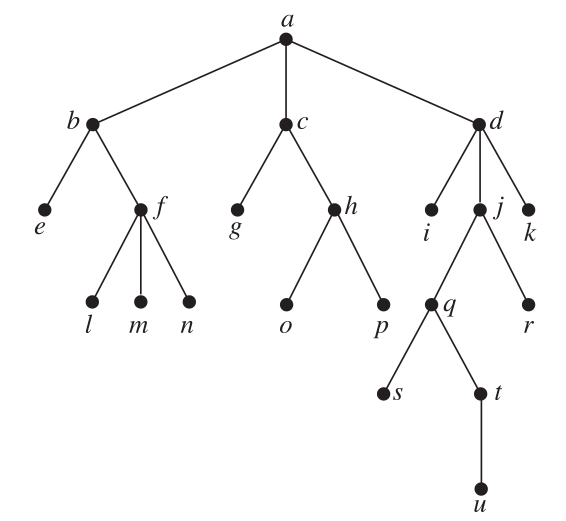
\includegraphics[width=200px]{assets/11,1,3.png}
				\label{}
				\caption{}
			\end{figure}
			\subsubsection{Which vertex is the root}
				$a$
			\subsubsection{Which vertices are internal}
				$b,c,d,f,h,j,q,t$
			\subsubsection{Which vertices are leaves}
				$e,l,m,n,g,o,p,i,k,r,s,u$
			\subsubsection{Which vertieces are children $j$}
				$q,r$
			\subsubsection{Which vertex is the parent $h$}
				$c$
			\subsubsection{Which vertices are siblings to $o$}
				$p$
			\subsubsection{Which vertices are ancestors of $m$}
				$f,b,a$
			\subsubsection{Which vertices are descendants of $b$}
				$e,f,l,m,n$
		\setcounter{subsection}{8}
		\subsection{Draw the tree from exercise 3 with root at:}
			\subsubsection{$a$}
			\begin{tikzpicture}
				[
					level 1/.style = {sibling distance = 4cm},
					level 2/.style = {sibling distance = 1.5cm}
				]
				\node{a}
					child{node{b}
						child{node{e}}
						child{node{f}
							child{node{l}}
							child{node{m}}
							child{node{n}}
						}
					}
					child{node{c}
						child{node{g}}
						child{node{h}
							child{node{o}}
							child{node{p}}
						}
					}
					child{node{d}
						child{node{i}}
						child{node{j}
							child{node{q}
								child{node{s}}
								child{node{t}
									child{node{u}}
								}
							}
							child{node{r}}
						}
						child{node{k}}
					};
		\end{tikzpicture}
			\setcounter{subsubsection}{2}
			\subsubsection{$e$}
				\begin{tikzpicture}
				[
					level 1/.style = {sibling distance = 4cm},
					level 2/.style = {sibling distance = 1.5cm}
				]
				\node{e};
			\end{tikzpicture}
		\setcounter{subsection}{13}
		\subsection{Show that a simple graph is tree if and only if it is connected but the deletion of any of its edges produces a graph that is not connected}
			For a simple graph to be a tree all the vertices has to be connected. A simple graph has no loops and therefore removing an edge will reuslt in it not being connected.
	
	\chapter{uge}
		\section{Afsnit 10.4}
			\setcounter{subsection}{11}
			\subsection{Determine whter each of these graphs is stringly connected and if not whter it is weakly connected}
				\begin{figure}[h!]
					\centering
					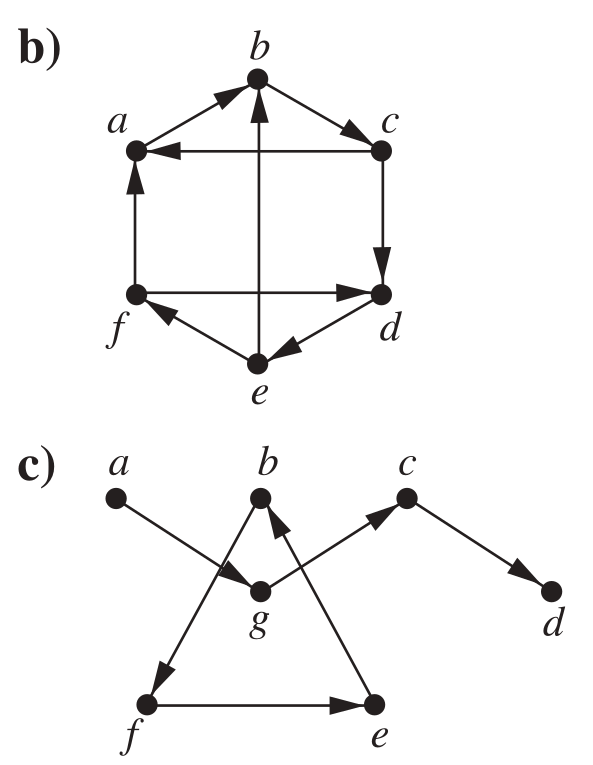
\includegraphics[width=250px]{assets/10,4,12,bc.png}
					\label{}
				\caption{Graphs for the following exercise}
				\end{figure}
				
				\setcounter{subsubsection}{1}
				\subsubsection{Strongly connectd}
				\subsubsection{Not connected}
			\setcounter{subsection}{13}
			\subsection{Find the strongly connnected componenets of each of these graphs}
				\begin{figure}[h!]
					\centering
					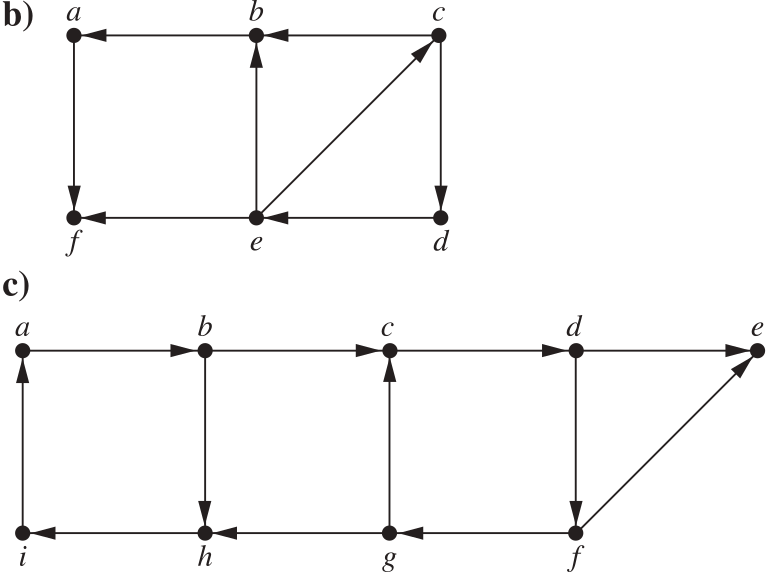
\includegraphics[width=250px]{assets/10,4,14,bc.png}
					\label{}
				\caption{Graphs for the following exercise}
				\end{figure}
				
				\setcounter{subsubsection}{1}
				\subsubsection{}
					$c,d,e,b,a,f$\\
					$f$\\
				\subsubsection{}
					$e$\\
					$a,b,c,d,f,g,h,i,e$
			\clearpage
			\section{Afsnit 11.1}
				\subsection{Which of these graphs are trees}
					\begin{figure}[h!]
						\centering
						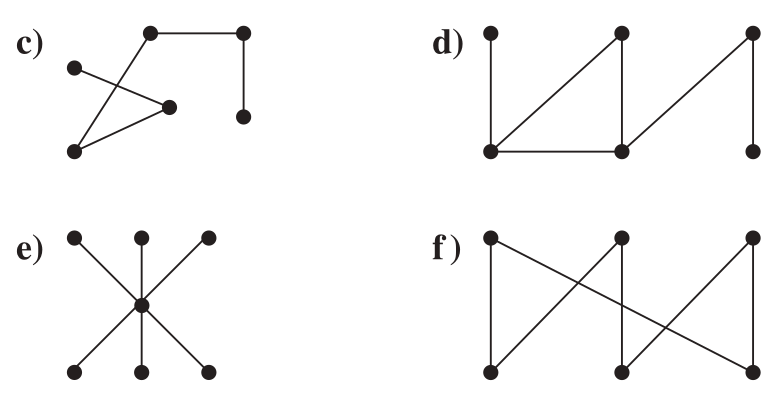
\includegraphics[width=250px]{assets/11,1,1,cef.png}
						\label{}
						\caption{}
					\end{figure}
					\setcounter{subsubsection}{2}
					\subsubsection{Yes}
					\setcounter{subsubsection}{4}
					\subsubsection{Yes}
					\subsubsection{No - its cyclic}
				\setcounter{subsection}{14}
				\subsection{Let $G$ be a simple graph with $n$ vertices. Show that}
					\subsubsection{$G$ is a tree if and only if it is connected and has $n-1$ edges}
						If it has $n$ edges then in the most simple example with two vertices it will create a cycle
					\subsubsection{$G$ is a tree if and onlu if $H$ has no simple circuits and has $n-1$ edges}
						For a graph to have simple circuit woul need a cycle to connect the circuit.
				\subsection{Which complete bipartite graphs $K_{m,n}$ where $m$ and $n$ are positive integers are trees?}
				$K_{1,n}\land K_{n,1}$ where $n\in\mathbb{N}$
			\setcounter{section}{0}
			\section{Afsnit 2.4}
				\subsection{Find these terms of the sequence $\{a_n\}$ where $a_n=2\cdot(-3)^n+5^n$}
					\subsubsection{$a_0$}
						$3$
					\subsubsection{$a_1$}
						$-1$
					\subsubsection{$a_4$}
						$787$
					\subsubsection{$a_5$}
						$2638$
				\setcounter{subsection}{8}
				\subsection{Find the first five terms of the sequence defined by each of these recurrence relations and initial conditiions}
					\subsubsection{$a_n=6a_{n-1},a_0=2$}
						\begin{align*}
							a_0&=2\\
							a_1&=12\\
							a_2&=72\\
							a_3&=432\\
							a_4&=2592\\
							a_5&=15552
						\end{align*}
					\subsubsection{$a_n=a_{n-1}^2,a_1=2$}
						\begin{align*}
							a_1&=2\\
							a_2&=4\\
							a_3&=16\\
							a_4&=256\\
							a_5&=65536
						\end{align*}
					\subsubsection{$a_n=a_{n-1}+3a_{n-2},a_0=1,a_1=2$}
						\begin{align*}
							a_0&=1\\
							a_1&=2\\
							a_2&=5\\
							a_3&=11\\
							a_4&=26\\
							a_5&=59
						\end{align*}
				\setcounter{subsection}{17}
				\subsection{A person deposits \$1000 in an account that yyeslds 9\% interest compunded annually}
					\subsubsection{Set up a recurrence relation for the amount in the account at the end of $n$ year}
						$a_0=1000$\\
						$a_n=a_{n-1}\cdot 1.09$
					\subsubsection{Find an explicit formula for the amount in the account at the end of $n$ years}
						$f(n)=1.09^n\cdot 1000$
					\subsubsection{How much money will the account contain after 100 years?}
						$f(100)=5.5\cdot 10^6$
				\setcounter{subsection}{28}
				\subsection{What are the values of these sums?}
				
					\subsubsection{$\sum\limits_{k=1}^5(k+1)$}
						$20$
					\subsubsection{$\sum\limits_{j=0}^4(-2)^j$}
						$11$
					\subsubsection{$\sum\limits_{i=1}^{10}3$}
						$3^10$
					\subsubsection{$\sum\limits_{j=0}^8(2^{j+1}-2^j)$}
						$511$
				\setcounter{subsection}{32}
				\subsection{Compute each of these double sums}
					
				\subsubsection{$\sum\limits_{i=1}^2\sum\limits_{j=1}^3(j+i)$}
					$30$
				\subsubsection{$\sum\limits_{i=1}^2\sum\limits_{j=1}^3(3j+2i)$}	
					$78$
				\setcounter{subsection}{44}
				\subsection{What are the values of the following products?}
					\subsubsection{$\Pi_{i=0}^{10}i$}
						36280
					\setcounter{subsubsection}{2}
					\subsubsection{$\Pi_{i=1}^{100}(-1)^i$}
						$-1$
			\section{$Adams, Essex$ afsnit 9.1}
			\subsection{Is the given sequence bounded, positive or negative, increasing, decreasing, or alternating, convergent, divergent, divergent to $\infty$ or $-\infty$}
					\subsubsection{$\{\frac{2n^2}{n^2+1}\}$}
						lower bound = 0\\
						upper bound = $\frac{1}{2}$\\
						positve\\
						increasing\\
						convergent
					\subsubsection{$\{\frac{2n}{n^2+1}\}$}
						Lower bound = -1\\
						Upper bound = 1\\
						convergent
				\subsection{Find the limit of the sequence if possible}
					\subsubsection{$a_n=\frac{5-2n}{3n-7}$}
						$-0.67$
					\subsubsection{$a_n=\frac{(n!)^2}{(2n)!}$}
						$0$
		\chapter{Uge}
			\section{Afsnit 2.4}
				\setcounter{subsection}{30}
				\subsection{2.4.31: What is the value of these sums of terms of a geometric progression?}
					\subsubsection{$\sum\limits_{j=0}^83\cdot 2^j$}
					\begin{align*}
						3\cdot \frac{r^{n+1}-1}{r-1}\\
						3\cdot \frac{2^{8+1}-1}{2-1}\\
						3\cdot \frac{2^9-1}{1}\\
						3\cdot 511\\
						1533
					\end{align*}
					\subsubsection{$\sum\limits_{j=1}^82^j$}
					\begin{align*}
						\frac{r^{n+1}-1}{r-1}-\frac{r^{n+1}-1}{r-1}\\
						\frac{2^9-1}{1}-\frac{2^1-1}{1}\\
						511-1\\
						510
					\end{align*}
				\subsection{Find the value of each of these sums}
					\setcounter{subsubsection}{2}
					\subsubsection{$\sum\limits_{j=0}^8(2\cdot 3^j+3\cdot 2^j)$}
					\begin{align*}
						3\cdot \frac{r^{n+1}-1}{r-1}+2\cdot \frac{r^{n+1}-1}{r-1}\\
						3\cdot \frac{2^{8+1}-1}{2-1}+2\cdot \frac{3^{8+1}-1}{3-1}\\
						3\cdot 511+2\cdot \frac{19682}{2}\\
						1533+19682\\
						21215
					\end{align*}
				\subsection{Compute each of these double sums}
					\setcounter{subsubsection}{2}
					\subsubsection{$\sum\limits_{i=1}^3\sum\limits_{j=0}^2i$}
						\begin{align*}
							\sum\limits_{i=1}^3(i+i+i)\\
							3\frac{3(3+1)}{2}\\
							18
						\end{align*}
					\subsubsection{$\sum\limits_{i=0}^2\sum\limits_{j=1}^3ij$}
						\begin{align*}	
							\sum\limits_{i=0}^2(i+2i+3i)\\
							\sum\limits_{i=0}^2(6i)\\
							6\cdot \frac{n(n+1)}{2}\\
							6\cdot \frac{2(3)}{2}\\
							18
						\end{align*}
				\setcounter{subsection}{38}
				\subsection{Find $\sum\limits_{k=100}^{200}k$}
					\begin{align*}
						\frac{n(n+1)}{2}-\frac{n(n+1)}{2}\\
						\frac{200(200+1)}{2}-\frac{100(100+1)}{2}\\
						20100-5050\\
						15050
					\end{align*}
				\setcounter{subsection}{44}
				\subsection{What are the values of the following produts}
					\setcounter{subsubsection}{1}
					\subsubsection{$\Pi_{i=5}^8i$}
						$5\cdot 6\cdot 7\cdot 8=1680$
					\setcounter{subsubsection}{3}
					\subsubsection{$\Pi_{i=1}^{10}2$}
							$2^{10}=1024$
				\subsection{Express $n!$ using product notation}
					$\prod\limits_{i=1}^n i$
			\section{Adams, Essex afsnit 9.1}
				\setcounter{subsection}{4}
				\subsection{Is the sequence bounded, positive or negative, increasing, decreasing or alternating or convergent/divergent}
					\subsubsection{$\{\frac{n^2-1}{n}\}$}
						lower bound - 0, increasing, divergent to $\infty$
					\subsubsection{$\{\frac{e^n}{\pi^n}\}$}
						lower bound -  0, decreasing, konvergent to 0
				\setcounter{subsection}{14}
				\subsection{Is it possible to limit the following sequences}
					\subsubsection{$a_n=\frac{n^2-4}{n+5}$}
						No limit
					\subsubsection{$a_n=\frac{n^22^n}{n!}$}
						Limit to 0
					\subsubsection{$a_n=\frac{\pi^n}{1+2^{2n}}$}
						Limit to 0
			\setcounter{section}{1}
			\section{Adams Essex afsnit 9.2}
			\subsubsection{$\sum_{n=1}^\infty\frac{1}{3^n}$}
				\begin{align*}
					\sum_{n=1}^\infty\frac{1}{3^n}\\
					\sum_{n=1}^\infty\frac{1}{3}(\frac{1}{3})^{n-1}\\
					\frac{1/3}{1-(1/3)}\\
					\frac{1}{2}
				\end{align*}
			\subsubsection{$\sum\limits_{n=1}^\infty\frac{3+2^n}{2^{n+2}}$}
				since the denominator is growing faster it will be lower and lower but will diverge to $\infty$
			\subsubsection{$\sum\limits_{n=1}^\infty\frac{1}{2n-1}$}
				The same argument it will diverge to $\infty$
	\chapter{Uge}
		\section{Adams, Essex afsnit 9.2}
			\setcounter{subsubsection}{3}
				\subsection{Is the sequence bounded, positive or negative, increasing, decreasing or alternating or convergent/divergent}
					$\sum\limits_{n=0}^{\infty}\frac{5}{10^{3n}}$\\
					$5\cdot \frac{1}{1-\frac{1}{1000}}=\frac{5000}{999}\approx 5.01$\\
					positve, decreasing, convergin to 0
			\setcounter{subsubsection}{15}
				\subsection{Is the sequence bounded, positive or negative, increasing, decreasing or alternating or convergent/divergent}
					$\sum\limits_{n=1}^{\infty}\frac{n}{n+1}$\\
					positive, increasing divergin to $\infty$ due to the fraction pretty much always being 1
			\setcounter{subsubsection}{17}
				\subsection{Is the sequence bounded, positive or negative, increasing, decreasing or alternating or convergent/divergent}
					$\sum\limits_{n=1}^{\infty}\frac{2}{n+1}$\\
					positve, increasing, divergin due to begin larger than $\frac{1}{n}$ which diverges
			\setcounter{subsubsection}{20}
			\subsubsection{When dropped an elastic ball bounces back up to a height three quaters of that from which it fell. If the ball is dropped form a height of 2 m and allwoed to bounce up and down indefinitely what is the total distance it travels before coming to rest?}
				$2+\sum\limits_{i=1}^{\infty}(\frac{3}{4})^i\cdot 4=2+4\cdot \frac{1}{1-\frac{3}{4}}-4=14$\\
		\setcounter{section}{0}
		\section{Adams Essex afsnit 9.2}
			\setcounter{subsection}{16}
			\subsection{Is the sequence bounded, positive or negative, increasing, decreasing or alternating or convergent/divergent}
				$\sum\limits_{n=1}^{\infty}n^{-1\frac{1}{2}}$\\
				positive, decreasing, diverges to $\infty$
			\setcounter{subsection}{22}
			\subsection{If a bank account pays 10\% simple interest into an account once a year, what is the balance in the account at then of 8 years if \$1,000 is deposited into the account at the beginning of each of the 8 years}
				$\sum\limits_{n=0}^8(1.1^n\cdot 1000-1000)=4570.48$
		\section{Adams Essex afsnit 9.3}
			\subsection{Does the term converge?}
				$\sum\limits_{n=1}^{\infty}\frac{1}{n^2+1}$\\
				It will converge to zero due to the denominator growing so fast
			\setcounter{subsection}{9}
			\subsection{$\sum\limits_{n=0}^{\infty}\frac{1+n}{2+n}$}
				Will diverge to $\infty$ due to $a$ never being 0 but always 1
			\subsection{$\sum\limits_{n=1}^{\infty}\frac{1+n^{4/3}}{2+n^{5/3}}$}
				\begin{align*}
					\lim\limits_{n\rightarrow \infty}\frac{\frac{1+n^{\frac{4}{3}}}{2+n^{\frac{5}{3}}}}{\frac{1}{n}}&=\lim\limits_{n\rightarrow \infty}\frac{n+n^{\frac{7}{3}}}{2+n^{\frac{5}{3}}}				\\
																				&=\lim\limits_{n\rightarrow\infty}\frac{\frac{1}{n^{\frac{2}{3}}}+n^{\frac{2}{3}}}{\frac{2}{n^{\frac{5}{3}}}+1} &&\text{Reduced by } n^{\frac{5}{3}}\\
																				&=\frac{0+\infty}{0+1}\\
																				&=0					
				\end{align*}
				Will converge to zero due to $n^{5/3}$ being faster growing
			\setcounter{subsection}{16}
			\subsection{$\sum\limits_{n=1}^{\infty}\frac{1}{2^n(n+1)}$}
				Will converge to zero
	\chapter{Uge}
		\section{Adams, Essex afsnit 9.3}
			\subsection{Does the series converge or diverge, use test}
				\setcounter{subsubsection}{1}
				\subsubsection{2 - $\sum\limits_{n=1}^{\infty}\frac{n}{n^4-2}$}
					$\frac{\frac{1001}{1001^4-2}}{\frac{1000}{1000^4-2}}=0.977$\\
					Konvergere
				\setcounter{subsubsection}{11}
				\subsubsection{12 - $\sum\limits_{n=1}^{\infty}\frac{n^2}{1+n\sqrt{n}}$}
					$\frac{\frac{1001^2}{1+1001\sqrt{1001}}}{\frac{1000^2}{1+1000\sqrt{1000}}}=1.0004$\\
					Diverge to $\infty$
				\setcounter{subsubsection}{17}
				\subsubsection{18 - $\sum\limits_{n=1}^{\infty}\frac{n^4}{n!}$}
					$\frac{\frac{1001^4}{1001!}}{\frac{1000^4}{1000!}}=0.001$\\
					Converge hard!			
				\subsubsection{19 - $\sum\limits_{n=1}^{\infty}\frac{n!}{n^2e^n}$}
					$\frac{\frac{1001!}{1001^2e^{1001}}}{\frac{1000!}{1000^2e^{1000}}}=367$\\
					Diverge
				\setcounter{subsubsection}{22}
				\subsubsection{23 - $\sum\limits_{n=1}^{\infty}\frac{(2n)!}{(n!)^3}$}
					$\frac{\frac{(2\cdot 1001)!}{(1001!)^3}}{\frac{(2\cdot 1000)!}{(1000!)^3}}=0$\\
					Converge
				\setcounter{subsubsection}{24}
				\subsubsection{25 - $\sum\limits_{n=1}^{\infty}\frac{2^n}{3^n-n^3}$}
					$\frac{\frac{2^{1001}}{3^{1001}-1001^3}}{\frac{2^{1000}}{3^{1000}-1000^3}}=0.67$\\
					Converge
\end{document}	

